\documentclass[11pt, oneside, dvipdfmx]{book}

\newcommand{\folder}{/usr/local/share/texmf}
%\newcommand{\folder}{/home/hanchenggao/Documents/texmf}
\input{\folder/hfiles/ebook}
\renewcommand{\thesubsubsection}{\Alph{subsubsection}.}
\setcounter{secnumdepth}{3}
%\usepackage[ruled,vlined]{algorithm2e}
\usepackage {graphicx}[dvips]
%\usepackage {graphics}
%\setCJKmainfont{SimSun}
\title{
A Novel Method for Obtaining the Structure of RTZ Inputs and their Corresponding Parity-Check Sequences: A First Step Towards Interleaver Design}
\author{Kwame Ackah Bohulu}
\date{\today}
\begin{document}

\maketitle
\section{Abstract}
The knowledege of the distance spectrum, as well as the structure of the message inputs that make up the distance spectrum for a specific Recursive Systematic Convolutional (RSC) code is vital to the design of Turbo Code interleavers. Whiles the distance spectrum of a RSC code can be obtained by calculationg its transfer function, it provides no information about the structure of the message inputs and the complexity involved in calculating the transfer function increases with the number of states of the RSC code.
%%%%%%%%%%%%%%%%%%%%%%%%%%%

In this paper,we present a novel low-complexity method for determining the distance spectrum of any RSC code which has the added benefit of revealing the structure of the message inputs that make up the distance spectrum.
%%%%%%%%%%%%%%%%%%%%%%%%%%%
 With the knowledge of the structure of the message inputs, we derive a general polynomial representation for them based on the weight of the message input after which we go a step further and derive corresponding parity-weight equations for the codewords they generate.
 %%%%%%%%%%%%%%%%%%%%%%
Finally, we compare the upper bound for both methods to simulation results and it is revealed that the upper bound obtained by the novel method is much tighter.
\section{Introduction}
A Convolutional Code (CC) is generated by passing an input message through a linear finite-state shift register. The structure of this code is such that it is best described using a trellis. This structure makes it possible to employ soft decision decoding algorithms, the most popular of these algorithms being the Viterbi algorithm. CC are used extensively in mobile communication and space communication application as a major component in concatenated code.  Depending on the configuration of the shift register being used to generate the code, a CC can either be \textit{recursive} or \textit{nonrecursive}. In the case of the recursive CC, a feedback shift register is used to generate the code. Furthermore if the input message appears in the CC, it is known as \textit{systematic}. Recursive Sytematic Convolutional (RSC) codes are used as component codes for turbo codes, which are one of the few error correcting codes with performance very close to the Shannon limit [1].

Low weight codeword are produced when the parity bit sequence has a very low weight. Amongst all such codewords, the one with the lowest weight determines the free distance $d_{\text{free}}$ of the code. 
$d_{\text{free}}$  of a RSC code is a very important factor and determines its error-correction performance [4].  This can be obtained from the distance spectrum of the RSC code which requires the calculation of the transfer function. The distance spectrum provides information about the number of codewords of weight $d$ generated by a message input of weight $w$. 
The message inputs are such that they diverge from and then return to the initial state, assuming edge effect is ignored. These message inputs are referred to as Return-To-Zero (RTZ) inputs and with respect to interleaver design for turbo codes, the structure of these inputs makes it possible to design good interleavers.
For this reason, the distance spectrum obtained as a result of the transfer function is not very useful, since it provides no information about the structure of the RTZ inputs. As an added downside, the complexity of calculating the transfer function for a given RSC code increases with the number of states.

In this paper,we present a novel alternate method to the Transfer Function whose complexity is independent of the number of states of the component code, and has the added benefit of making known the structure of the RTZ inputs that make up the distance spectrum.
With the knowledge of the structure of the message inputs, we derive a general polynomial representation for them based on the weight of the message input after which we go a step further and derive corresponding parity-weight equations for the codewords they generate.
 %%%%%%%%%%%%%%%%%%%%%%
Finally, we compare the upper bound for both methods to simulation results and it is revealed that the upper bound obtained by the novel method is much tighter.

The rest of the research paper is organised as follows. In Section \ref{sec2}, we give a brief review of RSC codes. In section \ref{sec3}, we describe how the distance spectrum of a RSC Code is obtained using the transfer function, followed by the presentation of our novel method in Section \ref{sec4}. Simulation results are presented in Section \ref{sec5} and we draw conclusions in Section \ref{sec6}
\section{Preliminaries}
binary vectors are represented by bold font and $\dot{\bv}$ represent an infinite repitition of the vector $\bv$ whiles $(\bv)_j$ represents the repitition of vector $\bv~j$ times   

$\bphi$ represent a primitive element in the extended Galois field GF($2^{\tau}$) and the vector representation for all elements in GF($2^{\tau}$) are written as $\bphi_i,~0 \leq i \leq 2^{\tau}$. 

The subscript $i$ represents the decimal value of the binary vector, which means $\bphi_0$ represents the all zero vector. All addition and multiplication operations are done in GF($2^{\tau}$).

The impulse response for a RSC code is given by $\btheta$ and the cycle of the RSC code and the associated cycle length is given by $\bpsi$ and $\tau$ respectively. $\btheta,~\bpsi$ and will be properly defined in the next section.
\section{Recursive Systematic Convolutional Codes:Review}
\label{sec2}

An $(n,k)$ RSC code is a convolutional code generated by using feedback shift registers which has its input bits as part of the codeword. At each time instant it receives an input of $k$ bits and outputs $n$ bits. The output bits are determined by the generator function, which may be written in polynomial notation as  $\Big[1 ~\frac{f(x)}{g(x)}\Big]$. Given the systematic nature of the RSC code, we only focus on the parity part of the RSC code and write the generator function simply as $\Big[\frac{f(x)}{g(x)}\Big]$ where $f(x)$ and $g(x)$ represent the feedfoward and feedback connections of the RSC encoder.  

It should be noted that the prescence of the feedback loop means that the code produced will have an infinite-length impulse response denoted $\btheta$. $\btheta$ is unique for each RSC code and it is the parity output when the input $(1~0~0~0~0~\cdots)$ is fed into the RSC encoder. Without having to feed the input into the encoder, we can find the impulse response as $\btheta=f(x)g^{-1}(x)$

  Within $\btheta$ is a vector $\bpsi$ (the cycle) that is repeated infinitely and the length of that cycle is represented by $\tau$.
 With the impulse response it is possible to calculate the parity weight generated by any input message. This is done by noting that each input message is a summation of shifted versions of the input $(1~0~0~0~0~\cdots)$ and therefore its parity-bit sequence is also a summation of shifted versions of the impulse response. This knowledge will be useful in the derivation of the parity weight equation for the RTZ inputs of a given RSC code.

Similar to any code, the minimum distance ($d_{\text{min}}$) of the RSC code also determines its error-correcting capability. With the aid of the distance spectrum, it is possible to determine $d_{\text{min}}$ as well as its multiplicity. The most common way to find the distance spectrum is via the transfer function of the RSC code. The transfer function enumerates all the paths that diverge from and then return to the initial state \cite{ref3}, ie the RTZ inputs. In other words, the distance spectrum provides information about the number of codewords of weight $d$ generated by an RTZ input of weight $w$. Combined with the knowledge that all RTZ inputs are divisible by $G(D)$ \cite{ref6}, we introduce a novel method for determining what we refer to as the  \textit{input structure distance spectrum} of any RSC code in the next section. This version of the distance spectrum is a better tool for interleaver design compared to the regular distance spectrum.

\begin{figure}[h]
\centering
		\includegraphics[width=0.45\textwidth]{./PaperSources/RSCExample3.pdf}
		\caption{$[\frac{1+x^2}{1+x+x^2}]$  RSC Encoder}
		\label{fig1}
		\end{figure}
		
A RSC encoder is shown in Figure \ref{fig1} with $k=1$ and $n=2$. Its generator function is given by $[\frac{1+x^2}{1+x+x^2}]$ which may be written as $5/7$ in octal form where $5 ~ \text{and} ~ 7$ correspond to the numerator and denomenator of the generator function respectively. 
 For the $5/7$ RSC code, $\btheta=(1~1~1~ 0~ 1~ 1~ 0~ 1~ 1~ 0~\cdots)$ which may be written in terms of the elements of GF(8) as $\bphi_7~\dot{\bphi_3}$. The corresponding cycle $\bpsi=\bphi_6 $ with a cycle length of $\tau =3$. 
 Moving foward all examples and discussions relating to RSC codes will be done using the $5/7$ RSC code unless otherwise stated.
 %The knowledge of $\textbf{p}$ and $\tau$ will be used in deriving the method for determing which input messages generate low-weight parity bits. 
\section{Distance Spectrum via Transfer Function of RSC Code}
\label{sec4}
The distance spectrum of an RSC code gives information about codeword weights and the number of codewords present in the code for a given weight generated as a result of message inputs that begin from, exit and then return to the zero state of the trellis of that code. Such message inputs are known as Return-to-Zero (RTZ) inputs. The distance spectrum of the RSC code can be obtained from its transfer function, denoted by $$T(Y,X)=\sum_{d=0}^{\infty}\sum_{w=0}^{\infty} a(d,w)Y^dX^w$$ where $a(d,w)$ is the number of codewords of weight $d$ generated by an input message of weight $w$.
Based on the method described in \cite{ref3}, we outline the process involved in deriving the transfer function of the $5/7$ RSC code. 

\begin{figure}[h]
\centering
		\includegraphics[width=0.45\textwidth]{tf.png}
		\caption{State Diagram of the $5/7$ RSC code }
		\label{Txfig4}
		\end{figure}
First, the state diagram of the $5/7$ RSC code is redrawn, as shown in Figure \ref{Txfig4}. The zero state is split into two and the transition from the zero state to itself is omitted. On each edge, the variables $Y^d$ and $X^w$ are used to represent the output weight $d$ and input weight $w$ of the path, respectively. We treat each edge label as a transfer block and employ the following rules for graph simplification:
Assume two edges labelled $H$ and $B$. Then,

\begin{enumerate}
\item If $H$ is connected in series to $B$, the labels are merged as $HB$.

\item If $H$ is connected in parallel to $B$, the labels are merged as $H+B$.

\item If the edges are in a feedback configuration, where $H$ and $B$ are the feedfoward and feedback portions respectively, the labels are merged as $\frac{H}{1-HB}$.
\end{enumerate}

In the following, we demonstrate the process for deriving the transfer function for the RSCC shown in Figure {\ref{Txfig4}}. The respective state diagram transformations are also shown in Figure {\ref{Txfig5}}.

\begin{figure}[h!]
\centering
		\includegraphics[width=0.5\textwidth]{tfexample.png}
		\caption{State Diagram Transformations involved in Transfer Function Calculation }
		\label{Txfig5}
		\end{figure}

\begin{example} Define all edge labels\\
\label{ex3}
 edge $ a\triangleq 0 0 \rightarrow 1 0$,  edge $b \triangleq 1 0 \rightarrow 0 1$\\
 edge $ c \triangleq 0 1 \rightarrow 0 0$, edge $d \triangleq 0 1 \rightarrow 1 0$\\
 edge $ e \triangleq 1 0 \rightarrow 1 1$, edge $f \triangleq 1 1 \rightarrow 1 1$\\
 edge $ g \triangleq 1 1 \rightarrow 1 0$

\begin{enumerate}
\item Simplify edge $g$ with feedback configuration

$$ \frac{1}{1-YX}$$

\item Merge edges $e,f,g$ with series configuration and rename it edge $h$

$$\text{edge}~h = Y\times \frac{1}{1-YX}\times Y=\frac{Y^2}{1-YX}$$

\item Merge edges $h,b$ with parallel configuration and rename it edge $j$

$$\text{edge}~j = YX+ \frac{Y^2}{1-YX}= \frac{YX+Y^2X^2+Y^2}{1-YX}$$

\item Merge  edges $j,d$ with feedback configuration and rename it edge $k$ 
\begin{equation*}
\begin{split}
 \text{edge}~k&= \frac{\frac{YX+Y^2X^2+Y^2}{1-YX}}{1-(\frac{YX+Y^2X^2+Y^2}{1-YX})}\\
 &=\frac{Y(X-YX^2+Y)}{1-2YX+Y^2X^2-Y^2}
\end{split}
\end{equation*}

\item Calculate transfer function by merging edges $k,a,c$ with series configuration

\begin{equation*}
\begin{split}
T(Y,X)&=Y^2X \times \frac{Y(X-YX^2+Y)}{1-2YX+Y^2X^2-Y^2}\times Y^2X \\
&=\frac{Y^5X^2(Y-YX^2+Y)}{1-2YX+Y^2X^2-Y^2}\\
&=Y^5X^3+Y^6(X^4+X^2)+Y^7(X^5+3X^3)+\\
&Y^8(X^6+6X^4+X^2)+Y^9(X^7+10X^5+5X^3)+...
\end{split}
\end{equation*}
\end{enumerate}
\end{example}

From the example, it is clear that the complexity involved in deriving the transfer function increases as the number of states of the RSCC increases and other methods such as Mason's Rule \cite{ref3} have to be used. Also to obtain the distance spectrum requires an extra division operation. In the case of interleaver design for Turbo codes, this method for generating the distance spectrum is not particularly useful. This is because it reveals no extra details with respect to the structure of the RTZ inputs. In the next section, we present a novel method whose complexity is independent of the number of states in the RSC code. As an added bonus, information regarding the structure of the RTZ inputs can be obtained using this method.
\section{Input-Structure Distance Spectrum }
\label{sec4}
The regular distance spectrum is an insufficient tool where it relates to interleaver design. In this section, we present a novel method that generates what we refered to as the input-structure distance spectrum. It is the distance spectrum with the structure of the RTZ inputs revealed making it a very useful tool for interleaver design.

For convinience sake we will switch to polynomial representation, where $g(x)$ and $f(x)$ represent the feedback and feedforward connections of the RSC code respectively. Also $b(x)$ and $h(x)$ are the polynomial representations of the input message and its corresponding parity-bit sequence respectively.

This method is simple and relies of the fact that a message input $b(x)$ is an RTZ input if 
\begin{equation}
b(x) \bmod g(x) =0
\label{eq1}
\end{equation}

Which means that we may rewrite $b(x)$ as $b(x)=a(x)g(x)$, where $a(x)$ is the polynomial representation of any binary vector or arbitrary length.

$h(x)$ is simply calculated as 
\begin{equation}
h(x) =a(x)f(x)
\label{eq2}
\end{equation}

With the above equations, finding the input-structure distance spectrum for an input message of length $N$ is as simple as using (\ref{eq1}) or  (\ref{eq2}) (or both ) for all values of $a(x),~x^0\in a(x), a(x) \in GF(2^N)$. The condition $x^0\in a(x)$ ensures that there is no repitition of $b(x)$ or $h(x)$

 For $N=16$ we find all $b(x) ~\text{and}~ h(x)$ for which $w_H(\textbf{h})=2 ~\text{and} ~ w_H(\textbf{h})=4$. The results are shown in Table \ref{tab1} and \ref{tab2} respectively . For $w_H(\textbf{h})=4$, only the first 10 results are shown.
 Also \ref{tab3} shows all $b(x)$ and $h(x)$ that produce a codeword weight $w_H(\bc) \leq 8$ for $N=32$.


 
    \begin{table*}[h]
 
 \caption{codewords with parity bit sequence weight $w_H(\textbf{h})=2$}
\centering
 \begin{tabular}{c c c} 
 \hline
 $w_H(\textbf{b})$ & $b(x)$ & $h(x)$ \\ [0.5ex] 
 \hline\hline
 3 &  $1+x+x^2$ & $1+x^2$\\ 
 4 & $1+x+x^3+x^4$ & $1+x^4$ \\
 5 & $1+x+x^3+x^5+x^6$ & $1+x^6$ \\
 6 & $1+x+x^3+x^5+x^7+x^8$& $1+x^8$ \\
 7 & $1+x+x^3+x^5+x^7+x^9+x^{10}$ & $1+x^{10}$ \\
 8 & $1+x+x^3+x^5+x^7+x^9+x^{11}+x^{12}$ & $1+x^{12}$\\ 
 9 & $1+x+x^3+x^5+x^7+x^9+x^{11}+x^{13}+x^{14}$ & $1+x^{14}$ \\ [1ex] 
 \hline
 \end{tabular}
 \label{tab1}
\end{table*}
 
 \begin{table*}[h!]
 
 \caption{codewords with parity bit sequence weight $w_H(\textbf{h})=4$}
\centering
 \begin{tabular}{c c c} 
 \hline
 $w_H(\textbf{b})$ & $b(x)$ & $h(x)$ \\ [0.5ex] 
 \hline\hline
 2 &  $1+x^3$ & $1+x+x^2+x^3$\\ 
 \hline 
  & $1+x^2+x^4$ &  $1+x+x^3+x^4$ \\
   3 &  $1+x^4+x^5$ & $1+x+x^2+x^5$ \\
  &  $1+x+x^5$ & $1+x^3+x^4+x^5$ \\
  \hline 
  & $1+x^2+x^3+x^5$ & $1+x+x^4+x^5$ \\
  &  $1+x^2+x^5+x^6$ & $1+x+x^3+x^6$ \\
 4 & $1+x^4+x^6+x^7$ & $1+x+x^2+x^7$\\ 
  &  $1+x+x^4+x^6$ & $1+x^{3}+x^5+x^6$ \\ 
  &  $1+x+x^6+x^7$ & $1+x^{3}+x^4+x^7$ \\  
  &  $1+x+x^3+x^7$ & $1+x^5+x^6+x^7$ \\ 
 [1ex]
 \hline
 \end{tabular}
 \label{tab2}
\end{table*}

\begin{table*}[h!]
 \caption{All $b(x)$ which produce codewords with weight $w_H(\bc) \leq 8$ for $M=32$}
\centering
 \begin{tabular}{c c c} 
 \hline
 $w_H(\textbf{c})$ & $b(x)$ & $h(x)$ \\ [0.5ex] 
 \hline\hline
 5 &  $1+x+x^2$ & $1+x^2$\\ 
 \hline 
  & $1+x^3$ &  $1+x+x^2+x^3$ \\
   6 &  $1+x+x^3+x^4$ & $1+x^4$ \\
  \hline 
  & $1+x^2+x^4$ & $1+x+x^3+x^4$ \\
  &  $1+x+x^5$ & $1+x^3+x^4+x^5$ \\
 7 & $1+x^4+x^5$ & $1+x+x^2+x^5$\\ 
  &  $1+x+x^3+x-5+x^6$ & $1+x^6$ \\ 
  \hline
  &$1+x^2+x^3+x^5$ & $1+x+x^4+x^5$ \\
  & $1+x^6$ & $1+x+x^2+x^4+x^5+x^6$\\
  & $1 +x +x^4+x^6$ & $1+x^3+x^5+x^6$ \\
  & $1 +x^2 +x^5 +x^6$ & $1+x+x^3+x^6$\\
  8 & $1+x+x^3+x^7$ & $1+x^5+x^6+x^7$ \\
  & $1+ x+x^6+x^7$ & $1+x^3+x^4+x^7$\\
  & $1+x^4+x^6+x^7$ & $1+x+x^2+x^7$\\
  & $1 +x +x^3 +x^5 +x^7 +x^8$ & $1+x^8$\\
 [1ex]
 \hline
 \end{tabular}
 \label{tab3}
\end{table*}
\section{Simulation Results}
Figures \ref{simFig1}, \ref{simFig2} and \ref{simFig3} show the comparison of the bounds obtained via our novel method to bounds obtained using the transfer function method as well as simulation results. For each RSC code, the codeword is BPSK modulated and transmitted over the AWGN channel. At the receiver end, the Viterbi Algorithm is used to decode before a decision is made on the decoded sequence.

\begin{figure}[h]
\centering
		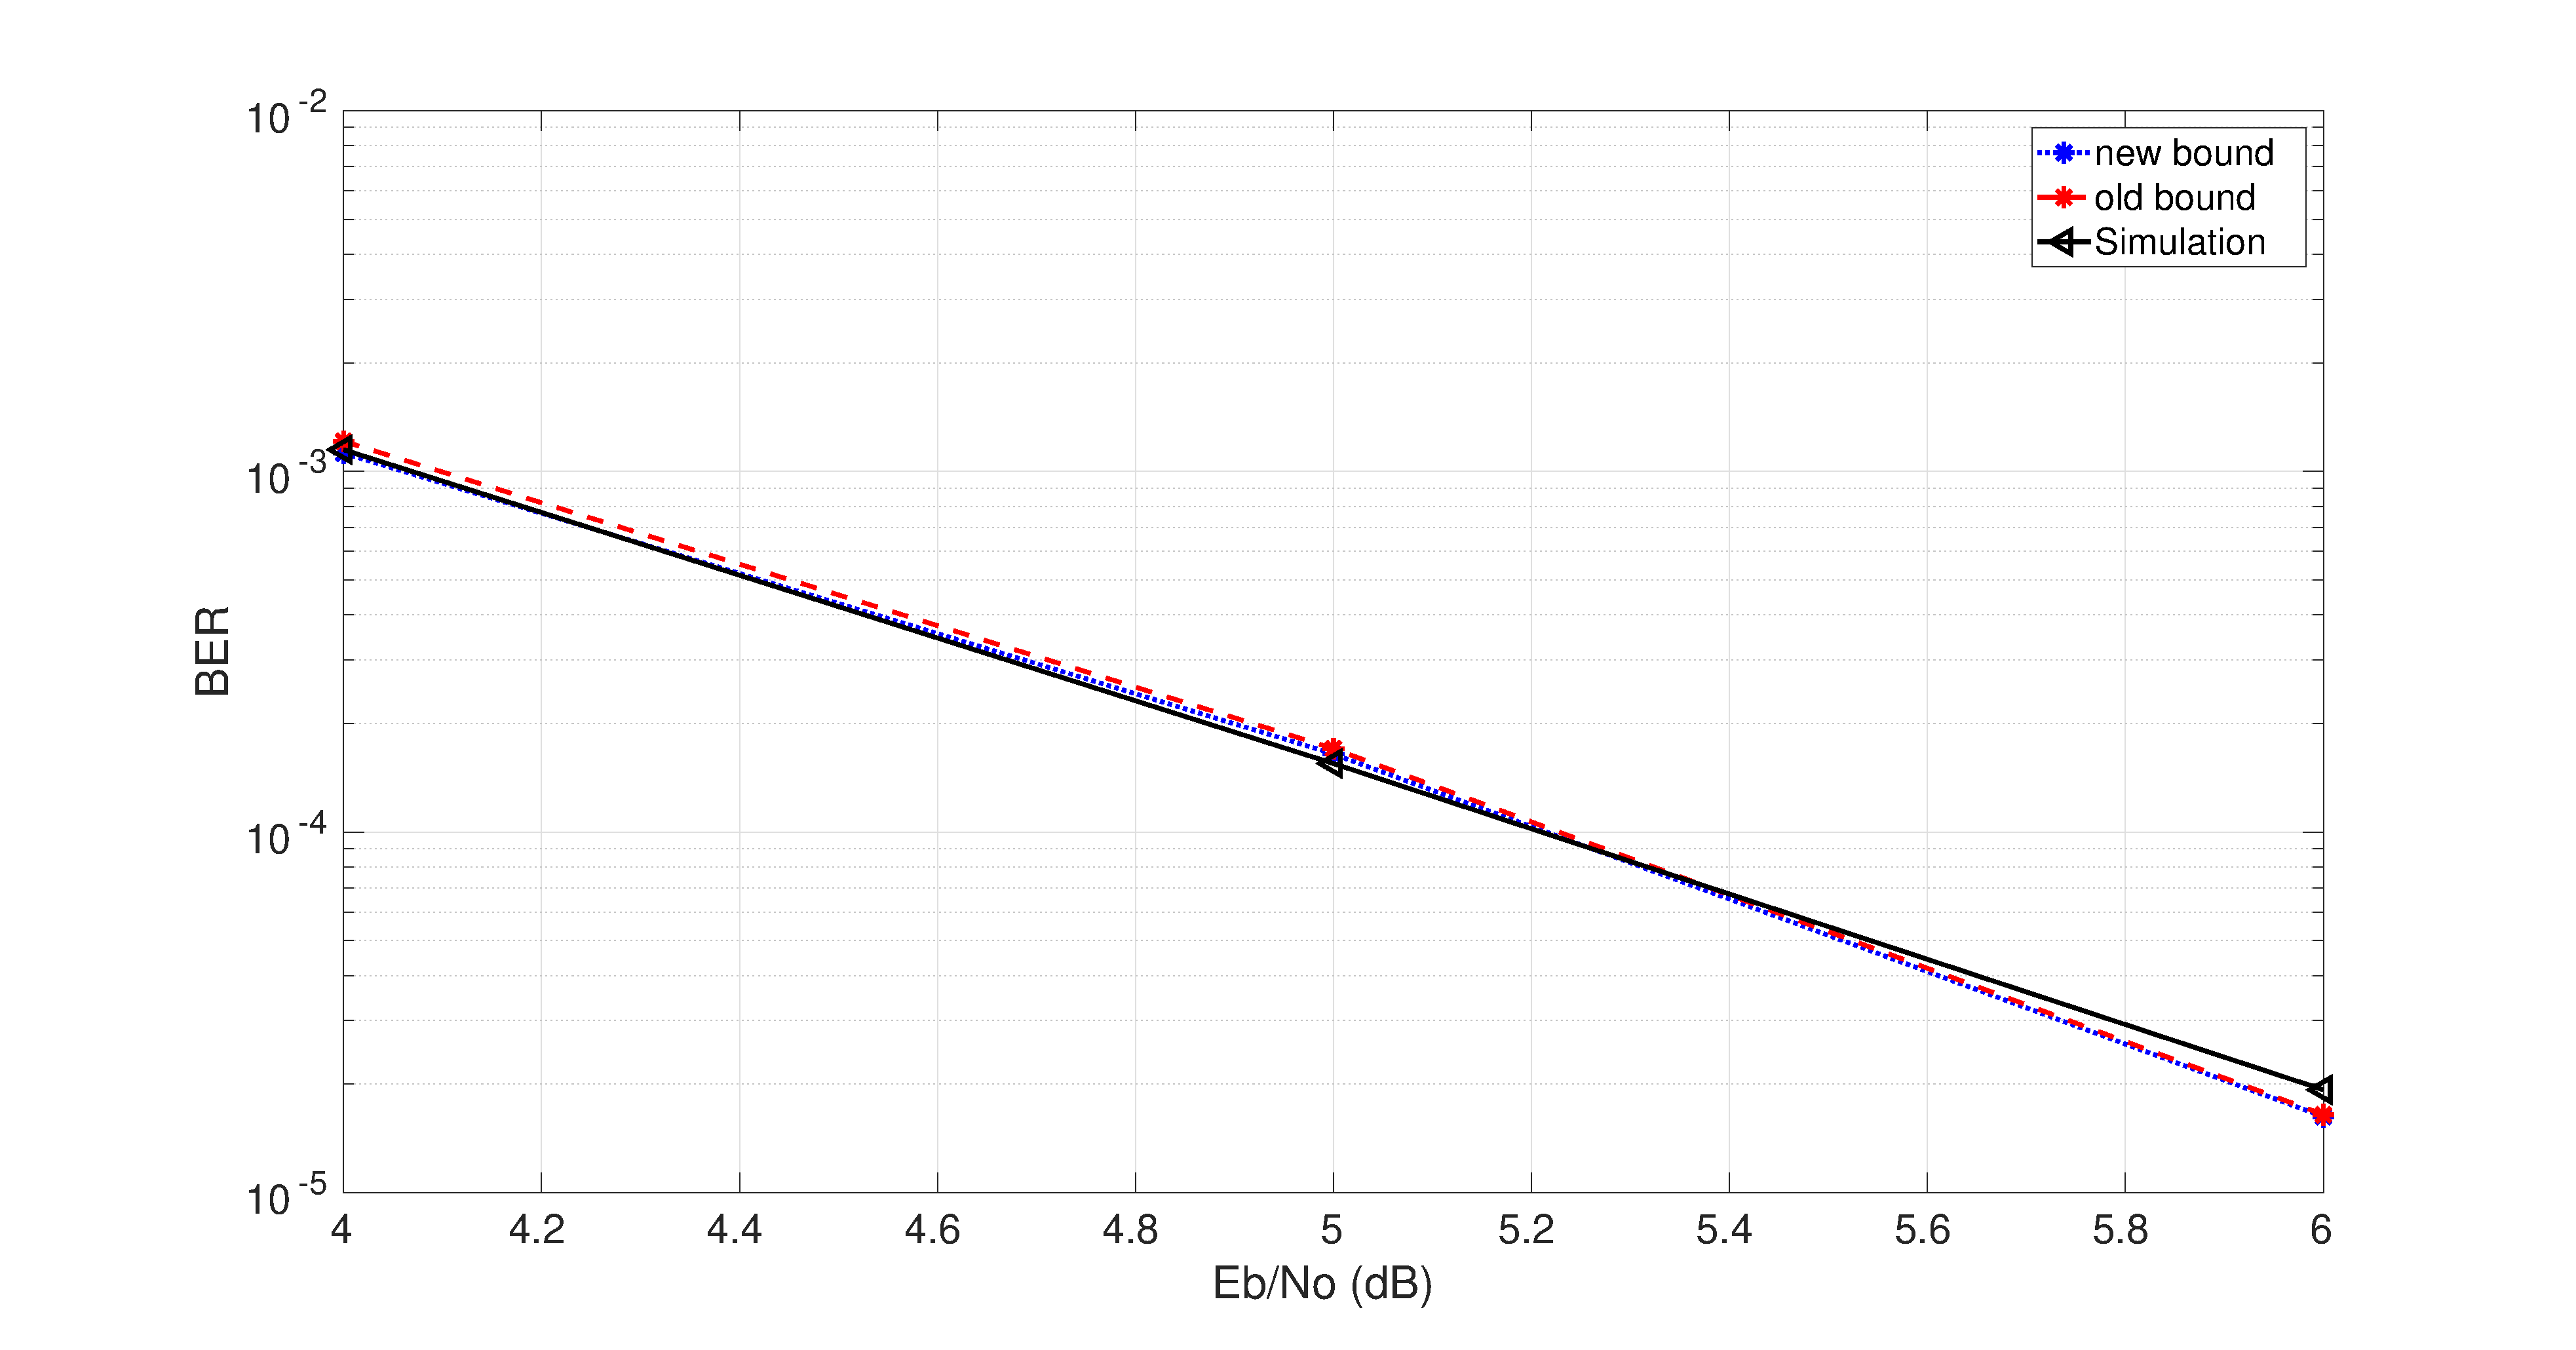
\includegraphics[width=0.5\textwidth]{./Images/RSC_5_7_v3.eps}
		\caption{Old Bound vs New Bound vs Simulation for 5/7 RSC Code}
		\label{simFig1}
		\end{figure}


\begin{figure}[h]
\centering
		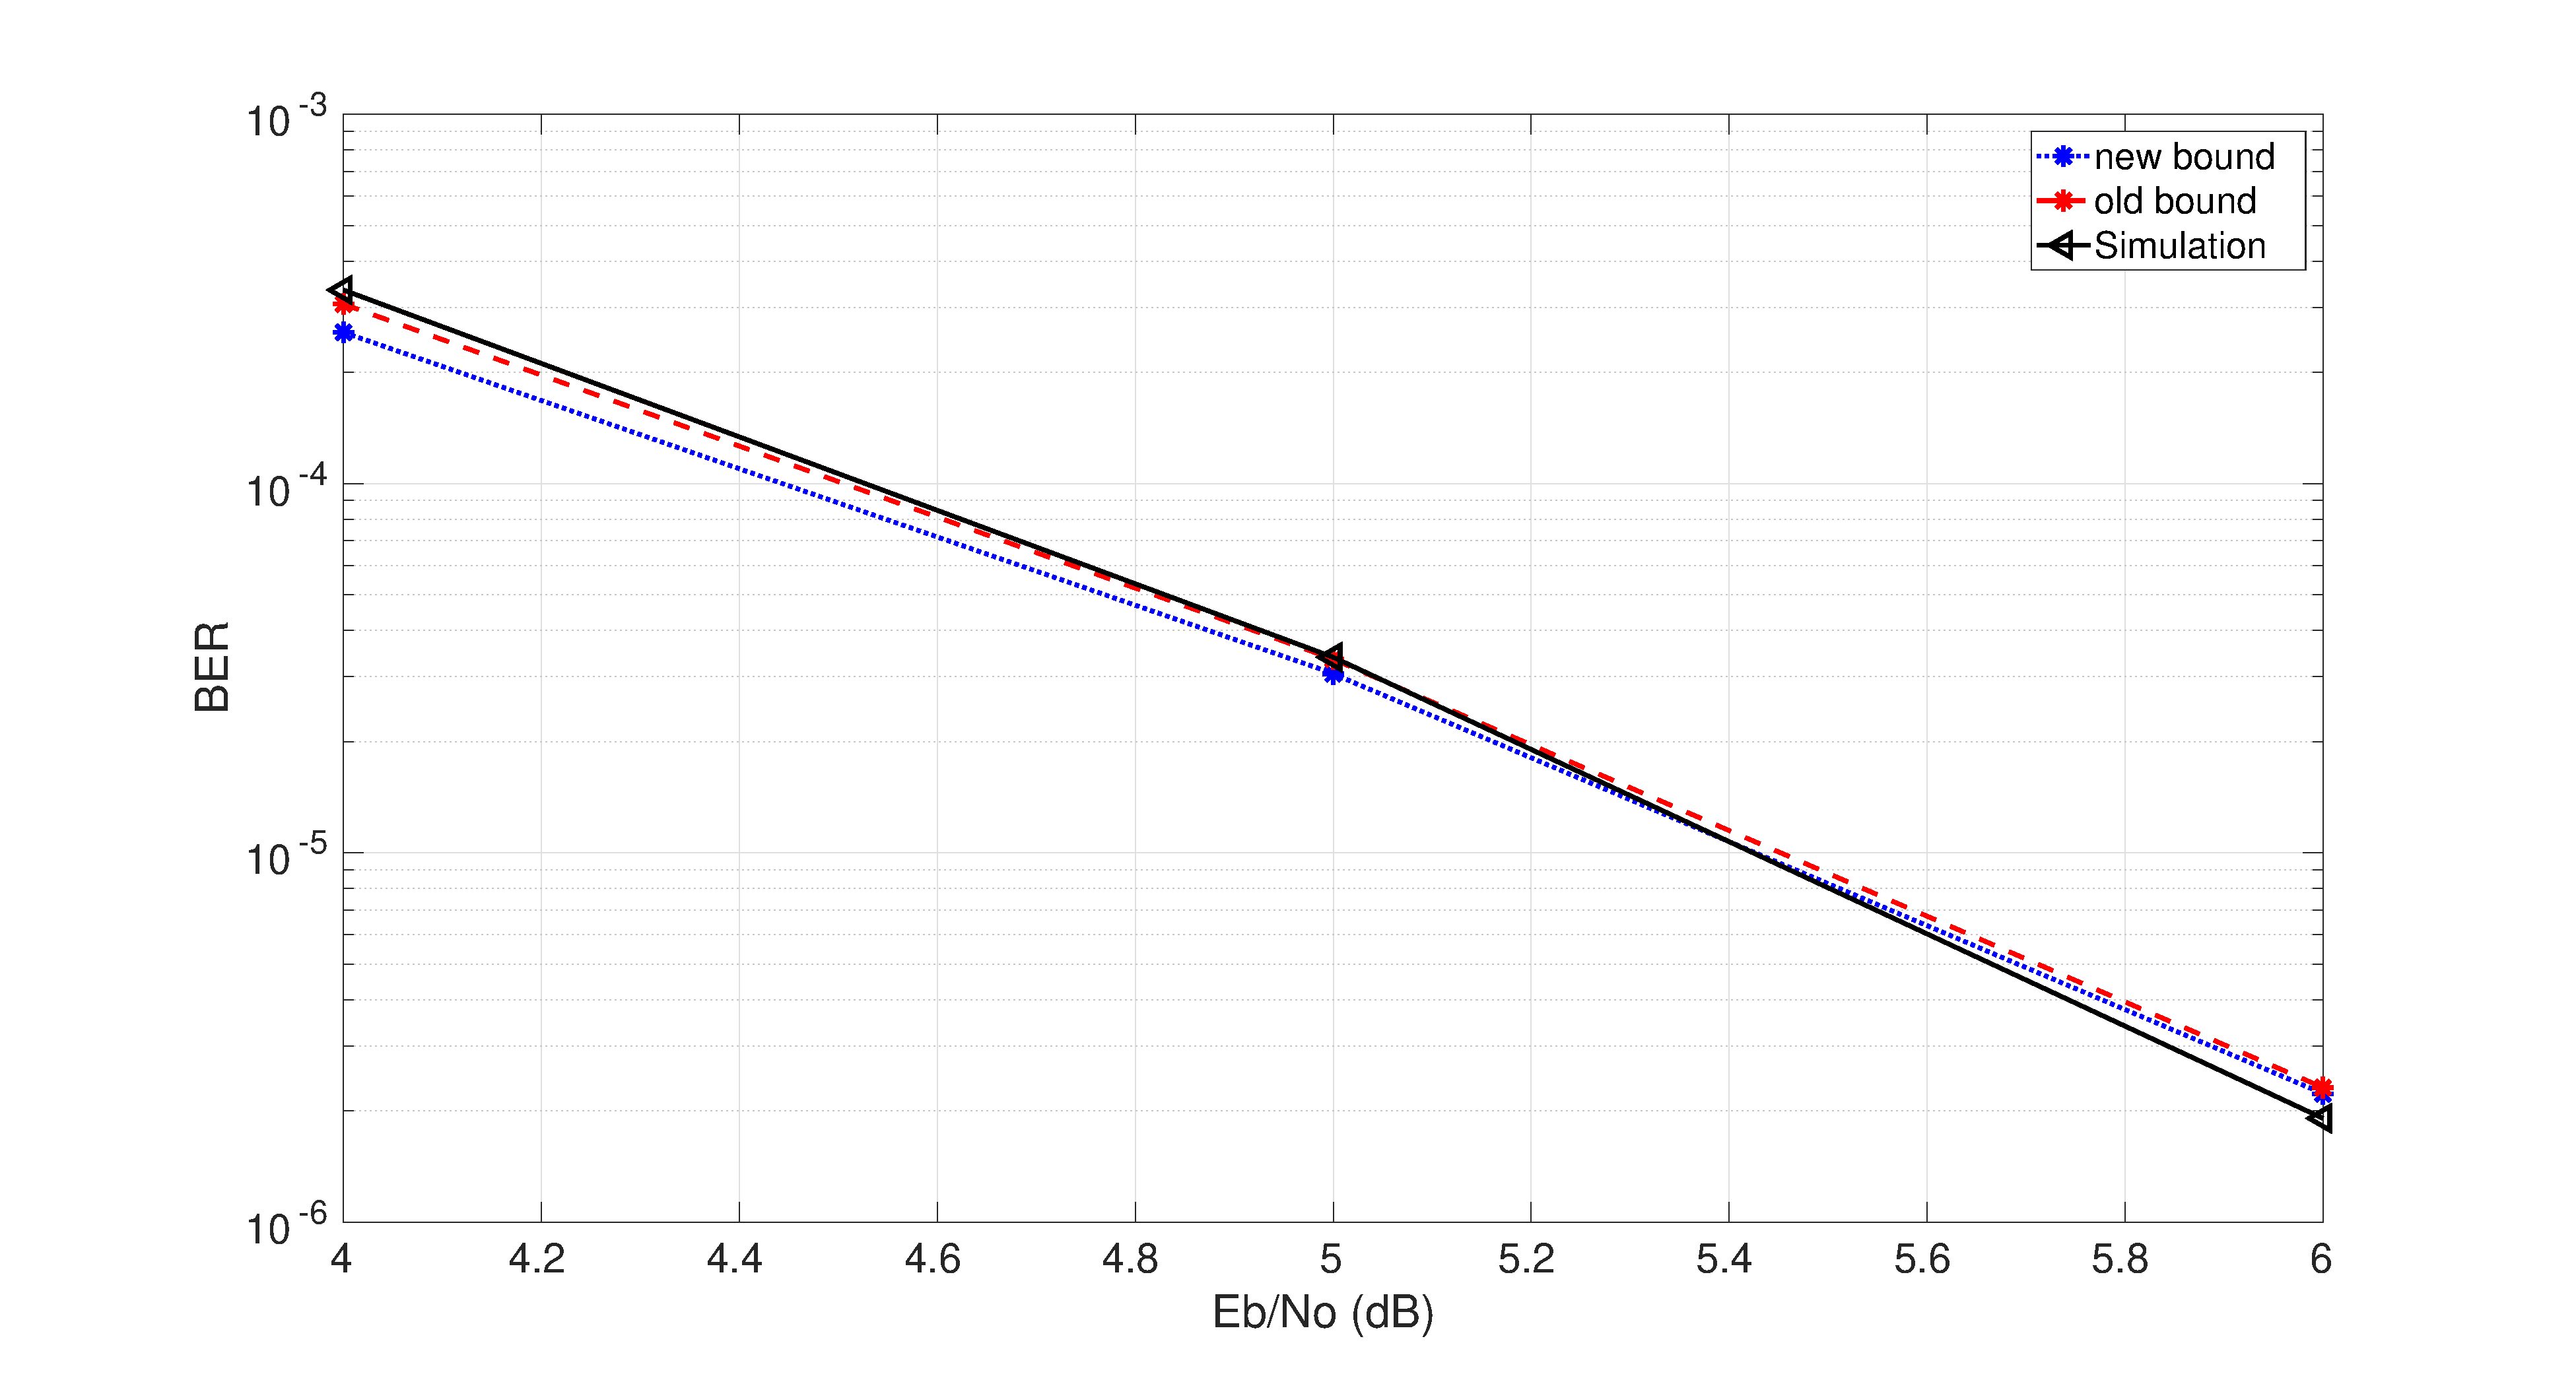
\includegraphics[width=0.5\textwidth]{./Images/RSC_37_21_v2.eps}
		\caption{Old Bound vs New Bound vs Simulation for 37/21 RSC Code}
		\label{simFig2}
		\end{figure}




%\section{Generalization of RTZ inputs and Their Corresponding Parity-Weight Equations}
With our method described in the previous section, we are able to not only determine the distance spectrum of the RSC code, but we have information with regards to the structure of the RTZ inputs. In this section, provide general information with regards to the type of RTZ inputs present in a RSC code. Then, we go a step further and provide a general representation (in polynomial form) of the RTZ inputs grouped by their weight. Finally we derive equations for calculating the parity weight for these RTZ inputs. The generalization as well as the derived equations will be very useful when it comes to designing interleavers for turbo codes.

%\subsection{Preliminaries}
%To aid in our proofs the following have been defined with respect to the impulse response of the $5/7$ RSC code.
%Let 
%\begin{eqnarray}
%&\bphi_1=(0~0~1)&,~\bphi_2=(0~1~0),~\bphi_4=(1~0~0)\\
%&\bphi_3=(0~1~1)&,~\bphi_6=(1~1~0),~\bphi_5=(1~0~1)\\
%&\bphi_7=(1~1~1)&
%\end{eqnarray}

%To simplify calculation, we have included an addition table for all the vectors which is shown in Table \ref{tb6-1}

%\begin{table}[h!]
%\centering
%\begin{tabular}{c || c  | c  | c  | c  | c  | c  | c } 
 %$$ & $\bphi_1$ & $\bphi_2$ & $\bphi_4$ & $\bphi_3$ & $\bphi_6$ & $\bphi_5$ & $\bphi_7$ \\
   %\hline\hline
  % %row1
%$\bphi_1$ & $\bphi_0$ & $-$ & $-$ & $-$ & $-$ & $-$ & $-$ \\
%   \hline
   %   %row2
%$\bphi_2$ & $\bphi_3$ & $\bphi_0$ & $-$ & $-$ & $-$ & $-$ & $-$ \\
  % \hline
  %    %row3
%$\bphi_4$ & $\bphi_5$ & $\bphi_6$ & $\bphi_0$ & $-$ & $-$ & $-$ & $-$ \\
%   \hline
  %    %row4
%$\bphi_3$ & $\bphi_2$ & $\bphi_1$ & $\bphi_7$ & $\bphi_0$ & $-$ & $-$ & $-$ \\
%   \hline
%      %row5
%$\bphi_6$ & $\bphi_7$ & $\bphi_4$ & $\bphi_2$ & $\bphi_5$ & $\bphi_0$ & $-$ & $-$ \\
%   \hline
%      %row6
%$\bphi_5$ & $\bphi_4$ & $\bphi_7$ & $\bphi_1$ & $\bphi_6$ & $\bphi_3$ & $\bphi_0$ & $-$ \\
%   \hline
%      %row7
%$\bphi_7$ & $\bphi_6$ & $\bphi_5$ & $\bphi_3$ & $\bphi_4$ & $\bphi_1$ & $\bphi_2$ & $\bphi_0$ \\
%   \hline
%  \end{tabular}
%\caption{Truth Table}
%\label{tb6-1}
%\end{table}

\subsection{Types of RTZ inputs}
Regardless of the component code used in turbo coding, the RTZ inputs can be grouped into two basic forms. We shall refer to them as \textit{base RTZ inputs} and \textit{compound RTZ inputs}. The number of base RTZ inputs depends on the component code and cannot be broken down into 2 or more RTZ inputs. Compound RTZ inputs as the name implies, are formed from 2 or more base RTZ inputs and therefore can be broken down into base RTZ input form.

For the $5/7$ component code, its base RTZ inputs are weight-$2$ RTZ inputs  (W2RTZs) and weight-$3$ RTZ inputs (W3RTZs). Every RTZ input with a weight higher than 3 is a compound RTZ input. In general for RTZs with weight $w$ greater than 3, if $w \bmod 2=0$, then the RTZ is made up of $w/2$ W2RTZs. On the other hand, if $w \bmod 2=1$, then the RTZ is made up of $\lfloor w/2 \rfloor -1$ W2RTZs and 1 W3RTZ.

%The impulse response of the RSC encoder is the output of the encoder when the input is $\brho=(1 0 0 0 0 ...)$. The impulse response can be used to calculate the weight of any input sequence of weight $w$ in general. This is done by noting that any input sequence of weight $w$ is just a summation of $w$ $\brho$'s, where the consequetive $w-1$ $\brho$'s have leading zeros. 
%For the 5/7 RSC encoder, the impulse response is given by $$(1 1 1 0 1 1 0 1 1 0 ...)$$
%The permutation matrix that generates the set $\cN$ is given by 

%$$\Pi'=\begin{bmatrix} 0 & 1 & 2 \end{bmatrix}$$ 
%where $\Pi$ was used repeatedly untill all elements in $\cC^t$ are picked. From $\Pi$ we can derive the defintions for W2RTZs and W3RTZs as well as ways to break up such RTZs
\subsection{General Form of RTZ Inputs}
In literature for turbo codes, it has been shown as the weight of the inputs increases, it has less effect on the bound of the BER[reference needed]. For this reason, for any RSC, we will provide a generalization for at most the first 4 distinct (by weight) RTZ inputs in the distance spectrum. These generalizations are obtained from using our novel method to list all the RTZ inputs up to weight $w$ that generate a codeword with weight $\leq d$ and taking note of the pattern that exists. The examples shown here are done with respect to the $5/7$ RSC and the at the end of the section shows the generalization for a few other RSC codes.

\subsubsection{General Form of W2RTZs}
A W2RTZ has the general form
\begin{equation}
\begin{split}
P(x)&=x^{h\tau+t}(1+x^{\alpha \tau})\\
& = x^t(x^{h\tau}+x^{(h+\alpha)\tau})
\end{split}
\end{equation}
where
$$h=0,1,2,...,\Big\lfloor \frac{M}{\tau} \Big\rfloor-1,~
 \alpha=1,2,...,\Big\lfloor \frac{M}{\tau} \Big\rfloor-h,~
 t=(0,1,...,\tau-1)$$

\begin{proof}
The proof will be to show that any polynomial of this form is an RTZ input. This can be done either by dividing $P(x)$ by $g(x)$ or by using the impulse response
\paragraph{division by g(x)}
Without loss of generality, we can assume that $h=t=0$ and $P(x) = 1+x^{\alpha \tau}$.
For any value of $\alpha,~P(x) \bmod g(x) = 0$ is always true. This proves that $P(x)$ is a RTZ input which has weight $2$.

\paragraph{Using the impulse response}
If we write $P(x)$ in binary for we have a summation of vectors that take the form
\begin{eqnarray*}
(\bphi_0~\bphi_1~(\bphi_6)_{\alpha-1}~\bphi_6~\cdots~\bphi_6)\cr
(\bphi_0~~(\bphi_0)_{\alpha}~~\bphi_1~\bphi_6~\cdots~\bphi_6)
\end{eqnarray*}
Regardless of the value of $\alpha$ we realize that there is an infinite summation of $\bphi_3+\bphi_3=\bphi_0$ after the second $1$ bit leading to a low-weight codeword, proving again that that $P(x)$ is a RTZ input which has weight $2$ or a W2RTZ.

This ends the proof.
\end{proof}

\subsubsection{General Form of W3RTZs}
A W3RTZ has the general form
\begin{equation}
\begin{split}
Q(x) &=x^{h\tau+t}(1+x^{\beta \tau +1}+x^{\gamma \tau +2})\\
&=x^{h\tau+t}+x^{(h+\beta) \tau +t+1}+x^{(h+\gamma) \tau +t+2}. 
\end{split}
\end{equation}
where
\begin{equation*}
\begin{split}
&h=0,1,2,...,\Big \lfloor \frac{M}{\tau} \Big\rfloor-1,~
\beta=0,1,2,...,\Big \lfloor \frac{M}{\tau} \Big\rfloor-1\\
&\gamma=0,1,2,...,\Big \lfloor \frac{M}{\tau} \Big\rfloor-1,~
 t=(0,1,...,\tau-1)
 \end{split}
 \end{equation*}
Notice that $h \leq \beta$ or $h \leq \gamma$ is not a necessary condition.
	
\begin{proof}
Similarly we prove that $Q(x)$ is a RTZ input either dividing $Q(x)$ by $g(x)$ or utilizing the impulse response. 
\paragraph{division by g(x)}
Without loss of generality, we can assume that $h=t=0$ and 
$Q(x) = 1+x^{\beta \tau +1}+x^{\gamma \tau +2}$.
For any value of $\beta~\text{and}~\gamma,~Q(x) \bmod g(x) = 0$ is always true. This proves that $Q(x)$ is a RTZ input which has weight $3$.

\paragraph{Using the impulse response}
If we write $Q(x)$ in binary for we have a summation of vectors that take the form
\begin{eqnarray*}
(\bzero_{3(\gamma+h)}~\bphi_1~\bphi_6~\cdots)\cr
(\bzero_{3(\beta+h)}~\bphi_3~\bphi_5~\cdots)\cr
(\bzero_{3 h}~~~~~~\bphi_7~\bphi_3~\cdots)
\end{eqnarray*}
Regardless of the value of $\beta$ and $\gamma$ we realize that there is an infinite summation of $\bphi_3+\bphi_3=\bphi_0$ after the third $1$ bit leading to a low-weight codeword, proving again that that $Q(x)$ is a RTZ input which has weight $3$ ie a W3RTZ.

This ends the proof.

\end{proof}.

\subsubsection{General Form of W4RTZs}
A W4RTZ has the general form
 \begin{equation}
 \begin{split}
  R(x)&=x^{h\tau+t}(1+x^{\alpha_1 \tau}) + x^{h'\tau+t'}(1+x^{\alpha_2 \tau})\\
  &= x^t(x^{h\tau}+x^{(h+\alpha_1)\tau}) + x^{t'}(x^{h'\tau}+x^{(h'+\alpha_2)\tau})
 \end{split}
 \end{equation}
	
where 
\begin{equation*}
\begin{split}
&h,~h'=0,1,2,...,\Big\lfloor \frac{M}{\tau} \Big\rfloor-1,~
 \alpha=1,2,...,\Big\lfloor \frac{M}{\tau} \Big\rfloor-h\\
& \alpha'=1,2,...,\Big\lfloor \frac{M}{\tau} \Big\rfloor-h',~
t,~t' \in\{0,1,..\tau-1\},h\tau+t \neq h'\tau+t'
\end{split}
\end{equation*}

It is obvious that the W4RTZ representation is valid since it is a combination of 2 W2RTZs

\subsubsection{W5RTZs : Definitions and Breaking them}
A W5RTZ has the general form
\begin{equation}
\begin{split}
 S(x)&=x^{h\tau+t}(1+x^{\alpha \tau}) 
	+
	x^{h'\tau+t'}(1+x^{\beta \tau +1}+x^{\gamma \tau +2})\\
	&= 
	x^t(x^{h\tau}+x^{(h+\alpha)\tau}) 
	+x^{h'\tau+t'}+x^{(h'+\beta) \tau +t'+1}+x^{(h'+\gamma) \tau +t'+2}
	\end{split}
	\end{equation}
	
where \begin{equation*}
\begin{split}
&h,~h'=0,1,2,...,\Big\lfloor \frac{M}{\tau} \Big\rfloor-1
,~\alpha'=1,2,...,\Big\lfloor \frac{M}{\tau} \Big\rfloor-h'\\
&\beta=0,1,2,...,\Big\lfloor \frac{M}{\tau} \Big\rfloor-1
,~\gamma=0,1,2,...,\Big\lfloor \frac{M}{\tau} \Big\rfloor-1\\
&t,~t' \in\{0,1,..\tau-1\},h\tau+t \neq h'\tau+t'
\end{split}
\end{equation*}

Again, it is obvious that the W4RTZ representation is valid since it is a combination of a W2RTZ and a W3RTZ.

\subsection{Parity Weight Equations for RTZ Inputs}
Once the general form of an RTZ input is know, we can calculate the parity weight of the codeword generated. In this section, we derive the equations for calculating the parity weight for the parity-bit sequences generated by those RTZ Inputs.

\subsubsection{Parity Weight Equations for W2RTZs}
The parity weight for a W2RTZ  $w^{(2)}_{p}$ is given by
\begin{equation}
w^{(2)}_{p}=2\alpha+2
\label{RTZinputs-1}
\end{equation}

\begin{proof}
For W2RTZ we consider the summation of the vectors below
\begin{eqnarray*}
(\bphi_1~\bphi_6~\cdots~\bphi_6~\bphi_6~\bphi_6~\bphi_6~\bphi_6\cdots~\bphi_6)\cr
+(\bphi_0~\bphi_0~\cdots~\bphi_0~\bphi_1~\bphi_6~\bphi_6~\bphi_6~\cdots~\bphi_6)\cr
\cline{1-2}
(\bphi_1~\bphi_6~\cdots~\bphi_6~\bphi'_3~\bphi_0~\bphi_0~\bphi_0~\cdots~\bphi_0)
\end{eqnarray*}

The derived vector will be 
\begin{equation*}
(\bphi_1~(\bphi_6)_{\alpha-1}~\bphi_7)
\end{equation*}

The parity weight $w_p^{(2)}$ is given by 
\begin{equation*}
\begin{split}
w_p^{(2)}&=2(\alpha-1)+4\\
&=2\alpha+2
\end{split}
\end{equation*}

This ends the proof.
\end{proof}

\subsubsection{Hamming Weight for W3RTZ Turbo Codewords }
The parity weight for a W3RTZ  $w^{(3)}_{p}$ is given by
\begin{equation}
2l+2
\label{RTZInputs-2}
\end{equation}
where $l=\max(\beta,\gamma)$
%=============proof begins=====================
\begin{proof}
$ $\newline
The polynomial representation of a weight-$3$ RTZ input is given by $$Q(x) =x^{h\tau+t}(1+x^{\beta \tau +1}+x^{\gamma \tau +2})$$
With reference to the impulse response of the 5/7  RSC encoder, 



Now, we consider the weight of the vector derived by the sumation of the followings vectors.
\begin{eqnarray*}
(\bzero_{3(\gamma+h)}~\bphi_1~\bphi_6~\cdots)\cr
(\bzero_{3(\beta+h)}~\bphi_3~\bphi_5~\cdots)\cr
(\bzero_{3 h}~~~~~~\bphi_7~\bphi_3~\cdots)
\end{eqnarray*}

Without loss of generality, we can assume that all weight-$3$ RTZ inputs begin at the $0$th position, ie $h=t=0$. This is because the case where $h>0$ or $t>0$ is just a right-shifted version of the weight-$3$ RTZ. With this assumption, we we only need to consider cases where $h= 0,~\gamma \geq h$.

Furthermore, we consider 4 general cases for all possible values of $i,j,k$ where $i \geq k$ These cases are $(=~=),~(=~<),~(<~=)$ and $(<~<)$
\paragraph{Case 0: $\gamma=\beta=h$ \newline}

 For this case, the vectors to sum will be 
 \begin{align*}
(\bphi_1~\bphi_6~\cdots)\\
(\bphi_3~\bphi_5~\cdots)\\
(\bphi_7~\bphi_3~\cdots)\\
\cline{1-2}
(\bphi_5~\bzero_{3}~\cdots)
\end{align*}
 
and  the derived vector will be $(\bphi_5~\bzero_{3}~\cdots)$ with a weight of $w_p=2$
 
 %========case =  < ===========
 
 %\paragraph{Case 1a: $i=j<k$\newline}
 %vector to sum:
 %\begin{align*}
 %(\bzero_{3}~\cdots~\bzero_{3}~\bphi_1~\bphi_6~\cdots~\bphi_3'~\bphi_3'~\bphi_3'~\cdots)\\
% (\bzero_{3}~\cdots~\bzero_{3}~\bphi_3~\bphi_5~\cdots~\bphi_5~\bphi_5\bphi_5~\cdots)\\
%+(\bzero_{3}~~\cdots~\cdots~\cdots~\cdots~\bzero_{3}~\bphi_7~\bphi_3~\cdots)\\
%\cline{1-2}
%(\bzero_{3}~\cdots~\bzero_{3}~\bphi_2~\bphi_3~\cdots~\bphi_3~\bphi_4~\bphi_0~\cdots)
%\end{align*}
%derived vector : $(\bzero_{3j}~\bphi_2~(\bphi_3)_{k-j-1}~\bphi_4~\bphi_0~\cdots)$
%\newline
%Parity weight: \begin{equation}
%\begin{split}
%w_p=2(k-j)
%\end{split}
%\end{equation}

\paragraph{Case 1a: $\gamma=h<\beta$ \newline}
 vectors to sum:
 \begin{align*}
(\bphi_1~\bphi_6~\bphi_6~\bphi_6~\bphi_6~\cdots)\\
(\bzero_{3}~\cdots~\bzero_{3}~\bphi_3~\bphi_5~\cdots)\\
+(\bphi_7~\bphi_3~\bphi_3~\bphi_3~\bphi_3~\cdots)\\
\cline{1-2}
(\bphi_6~\bphi_5~\bphi_5~\bphi_6~\bphi_0~\cdots)
\end{align*}
derived vector : $(\bphi_6~(\bphi_5)_{\beta-h-1}~\bphi_6~\bphi_0~\cdots)$
\newline
Parity weight: \begin{equation}
\begin{split}
w_p=2(\beta-h)+2 =2\beta+2
\end{split}
\end{equation}

\paragraph{Case 1b: $\beta=h<\gamma$\newline}
 vectors to sum:
\begin{align*}
(\bzero_{3}~\cdots~\cdots~\bzero_{3}~\bphi_1~\bphi_6~\cdots)\\
(\bphi_3~\bphi_5~\cdots~\bphi_5~\bphi_5\bphi_5~\cdots)\\
+(\bphi_7~\bphi_3~\cdots~\bphi_3~\bphi_3~\bphi_3~\cdots)\\
\cline{1-2}
(\bphi_4~\bphi_6~\cdots~\bphi_6~\bphi_7~\bphi_0~\cdots)
\end{align*}
derived vector : $(\bphi_4~(\bphi_3)_{\gamma-h-1}~\bphi_7~\bphi_0~\cdots)$\newline
Parity weight: \begin{equation}
\begin{split}
w_p=2(\gamma-h)+2=2\gamma+2
\end{split}
\end{equation}

\newpage
\paragraph{Case 2a: $h<\gamma=\beta$ \newline}
 vectors to sum:
\begin{align*}
(\bphi_0\cdots~\cdots~\bphi_0~\phi_1~\phi'_2~\cdots)\\
(\bphi_0\cdots~\cdots~\bphi_0~\phi_2~\phi''_2~\cdots)\\
+(\phi_3~\phi_2~\cdots~\phi_2~\phi_2~\phi_2~\cdots)\\
\cline{1-2}
(\bphi_7~\bphi_3~\cdots~\bphi_3~\bphi_1~\bphi_0~\cdots)
\end{align*}


derived vector : $(\bphi_7~(\bphi_3)_{\gamma-h-1}~\bphi_1~\bphi_0~\cdots)$
\newline
Parity weight: \begin{equation}
\begin{split}
w_p=2(\gamma-h)+2 =2\gamma+2
\end{split}
\end{equation}
 
\paragraph{Case 3a: $h<\gamma<\beta$ \newline}
vectors to sum:
\begin{eqnarray*}
(\bphi_0\cdots\cdots~\bphi_0~\phi_1~\phi'_2~\cdots~\phi'_2~\phi'_2~\phi'_2\cdots)\cr
(\bphi_0\cdots~\cdots~\cdots~\cdots~\cdots~\bphi_0~\phi_2~\phi''_2\cdots)\cr
+(\phi_3~\phi_2~\cdots~\phi_2~\phi_2~\phi_2~\cdots~\phi_2~\phi_2~\phi_2\cdots)\cr
\cline{1-2}
(\bphi_7~\bphi_3\cdots~\bphi_3~\bphi_2~\bphi_5\cdots~\bphi_5~\bphi_6~\bphi_0\cdots)
\end{eqnarray*}


derived vector : $(\bphi_7~(\bphi_3)_{\gamma-h-1}~\bphi_2~(\bphi_5)_{\beta-\gamma-1}~\bphi_6~\bphi_0~\cdots)$
\newline
Parity weight: \begin{equation}
\begin{split}
w_p&=2(\gamma-h)+2+2(\beta-i)\\
&=2(\beta-h)+2\\
& = 2\beta+2
\end{split}
\end{equation}

\paragraph{Case 3b: $h<\beta<\gamma$\newline}
\begin{eqnarray*}
(\bphi_0~\cdots~\cdots~\cdots~\cdots~\cdots~\bphi_0~\phi_1~\phi'_2\cdots)\cr
(\bphi_0~\cdots\cdots~\bphi_0~\phi_2~\phi''_2~\cdots~\phi''_2~\phi''_2~\phi''_2\cdots)\cr
+(\phi_3~\phi_2~\cdots~\phi_2~\phi_2~\phi_2~\cdots~\phi_2~\phi_2~\phi_2\cdots)\cr
\cline{1-2}
(\bphi_7~\bphi_3\cdots~\bphi_3~\bphi_0~\bphi_6\cdots~\bphi_6~\bphi_7~\bphi_0\cdots)
\end{eqnarray*}
derived vector : $(\bphi_7~(\bphi_3)_{j-k-1}~\bphi_0~(\bphi_6)_{i-j-1}~\bphi_7~\bphi_0~\cdots)$\newline
Parity weight: \begin{equation}
\begin{split}
w_p &=2(\beta-h)+1 +2(\gamma-\beta)+1 \\
&=2(\gamma-h)+2\\
&=2\gamma+2
\end{split}
\end{equation}

From all the above cases we can conclude that the parity weight for a weight-$3$ RTZ sequence may be calculated as
\begin{equation}
w_p^{(3)}=
2l+2 
\end{equation}
where $l=\max( \gamma,\beta )$

This ends the proof
\end{proof}
%==============proof end==================
\subsubsection{Hamming weight for W4RTZ Turbo Codewords}
The parity weight for a W4RTZ  $w^{(4)}_{p}$ is given by

\begin{equation}
w_p^{(4)} =
\begin{cases}
2(\alpha+\alpha')+4, & \text{if}\ h\tau+t<(h+\alpha)\tau+t< h'\tau+t'<(h'+\alpha')\tau+t' \\
2(\alpha), & \text{if}\ h\tau+t< h'\tau+t'<(h'+\alpha')\tau+t'<(h+\alpha)\tau+t,~t\neq t' \\
2(\alpha' +(h'-h) +(t'-t)-1), & \text{if}\ h\tau+t< h'\tau+t'<(h+\alpha)\tau+t<(h'+\alpha')\tau+t' ,~t\neq t'
    \end{cases}
\label{RTZInputs-3}
\end{equation}



\begin{proof}
For all the proofs, we will rely on the parity vector for W2RTZs, which is given by
$$(\bphi_1~ (\bphi_6)_{\alpha-1}~ \bphi_7)$$
\paragraph{Case 1: $h\tau+t<(h + \alpha)\tau+t<h'\tau+t'<(h' + \alpha')\tau+t'$\newline}

For this case, we have the following parity vector summation.
\begin{eqnarray*}
(\bphi_1~ \bphi_6~ \bphi_6~\cdots~ \bphi_6~ \bphi_7~\cdots ~\bphi_0~\bphi_0~\bphi_0~\cdots~\bphi_0~\bphi_0~
\cdots~\bphi_0)\cr
+(\bphi_0~\bphi_0~\bphi_0~\cdots~\bphi_0~\bphi_0~\cdots~\bphi_1~ \bphi_6~ \bphi_6~\cdots~\bphi_6~ \bphi_7~\cdots~\bphi_0)\cr
\cline{1-2}
(\bphi_1~ \bphi_6~ \bphi_6~\cdots~ \bphi_6~ \bphi_7~\cdots~\bphi_1~ \bphi_6~ \bphi_6~\cdots~\bphi_6~ \bphi_7~\cdots~\bphi_0)
\end{eqnarray*}

The derived parity vector is then $(\bphi_1~ (\bphi_6)_{\alpha-1}~ \bphi_7~\cdots~\bphi_1~ (\bphi_6)_{\alpha'-1}~ \bphi_7)$ and the weight for the derived parity vector is calculated as 
\begin{equation}
\begin{split}
w_p=&2(\alpha)+2+2(\alpha')+2\\
=&2(\alpha + \alpha')+4
\end{split}
\end{equation}

\paragraph{Case 2: $h\tau+t<h'\tau+t'<(h' + \alpha')\tau+t'<(h + \alpha)\tau+t,~
t'\neq t$\newline}

For the above case, there are 3 possible vector summations as shown below

\paragraph{Case 2a\newline}
\begin{eqnarray}
(\bphi_1~ \bphi_6~\cdots~\bphi_6~ \bphi_6~ \bphi_6~\cdots~ \bphi_6~ \bphi_6~ \bphi_6~\cdots~ \bphi_6~\bphi_7)\cr
+(\bphi_0~~\bphi_0~\cdots~\bphi_0~\bphi_7~\bphi_3~\cdots~\bphi_3~\bphi_4~\bphi_0
~\cdots~\bphi_0~\bphi_0)\cr
\cline{1-2}
(\bphi_1~ \bphi_6~\cdots~\bphi_6~\bphi_1~\bphi_5~\cdots~\bphi_5~\bphi_2~\bphi_6~
\cdots ~\bphi_6~\bphi_7)
\label{2-1}
\end{eqnarray}
for Case 2a, the derived parity vector is $$(\bphi_1~ (\bphi_6)_{(h'-h)}~\bphi_1~(\bphi_5)_{(\alpha'-1)}~\bphi_1~(\bphi_6)_{((h-h')+(\alpha-\alpha')-2)}~\bphi_7)$$
with a corresponding weight of 
\begin{equation*}
\begin{split}
w_p&=2(h'-h)+1+2(\alpha'-1)+1+2((h-h')+(\alpha-\alpha')-2)+4\\
&=2(h'-h)+1+2\alpha'-1+2(h-h')+2(\alpha-\alpha')\\
&=2(\alpha'-\alpha'+\alpha)\\
&=2\alpha
\end{split}
\end{equation*}

\paragraph{Case 2b \newline}
\begin{eqnarray}
(\bphi_1~ \bphi_6~\cdots~ \bphi_6~ \bphi_6~ \bphi_6~\cdots~ \bphi_6~ \bphi_6~ \bphi_6~\cdots~\bphi_6~ \bphi_7)\cr
+(\bphi_0~~\bphi_0~\cdots~\bphi_0~\bphi_3~\bphi_5~\cdots~\bphi_5~
\bphi_6~\bphi_0~\cdots~\bphi_0
~\bphi_0)\cr
\cline{1-2}
(\bphi_1~ \bphi_6~\cdots~ \bphi_6~\bphi_5~\bphi_3~\cdots~\bphi_3~\bphi_0~\bphi_6~\cdots~\bphi_6 \bphi_7)
\label{2-2}
\end{eqnarray}
For Case 2b, the derived parity vector is $$
(\bphi_1~(\bphi_6)_{(h'-h)}~\bphi_5~(\bphi_3)_{(\alpha-1)}~\bphi_0~(\bphi_6)_{((h-h')+(\alpha-\alpha')-2)}~\bphi_7)
$$
And the parity weight is 
\begin{equation*}
\begin{split}
w_p&=2(h'-h)+1+2(\alpha'-1)+2+2((h-h')+(\alpha-\alpha')-2)+3\\
&=2(h'-h)+1+2\alpha'-2+2+2(h-h')+2(\alpha-\alpha')-1\\
&=2(\alpha'-\alpha'+\alpha)\\
&=2\alpha
\end{split}
\end{equation*}

\paragraph{Case 2c \newline}
\begin{eqnarray}
(\bphi_1~ \bphi_6~ \bphi_6~ \bphi_6~\cdots~ \bphi_6~ \bphi_6~ \bphi_6~ \bphi_7)\cr
+(\bphi_0~~\bphi_0~\bphi_1~ \bphi_6~\cdots~\bphi_6~ \bphi_7~\bphi_0
~\bphi_0)\cr
\cline{1-2}
(\bphi_1~ \bphi_6~\bphi_7~\bphi_0~\cdots~\bphi_0~\bphi_1~\bphi_6~ \bphi_7)
\label{2-3}
\end{eqnarray}

For Case 2c, $t=t'$ and the derived vector as well as the parity weight is the same as that of the Type1 W4RTZ.
Therefore for Case 2, the parity weight is given by
\begin{equation}
w_p=2\alpha 
\end{equation}

\paragraph{Case 3: $h\tau+t<h'\tau+t'<(h + \alpha)\tau+t<(h' + \alpha')\tau+t',~
t'\neq t $ \newline}
Similarly, there are 3 possible vector summations as shown below

\paragraph{Case 3a \newline}
\begin{eqnarray}
(\bphi_1~ \bphi_6~\cdots~ \bphi_6~ \bphi_6~ \bphi_6~\cdots~ \bphi_6~
 \bphi_7~\bphi_0~\cdots~\bphi_0~\bphi_0)\cr
+(\bphi_0~\bphi_0~\cdots~\bphi_0~\bphi_7~\bphi_3~\cdots~\bphi_3~\bphi_3
~\bphi_3\cdots~\bphi_3~\bphi_4)\cr
\cline{1-2}
(\bphi_1~\bphi_6~\cdots~\bphi_6~\bphi_1~\bphi_5~\cdots~\bphi_5~\bphi_4
~\bphi_3\cdots~\bphi_3~\bphi_4)
\label{3-1}
\end{eqnarray}

For Case 3a the derived parity vector is $$
(\bphi_1~(\bphi_6)_{(h'-h)}~\bphi_1~(\bphi_5)_{(h-h'+\alpha)-2}~\bphi_4~(\bphi_3)_{((h'-h)+(\alpha'-\alpha))}~\bphi_4)
$$
with a weight of 
\begin{equation*}
\begin{split}
w_p&=2(h'-h)+1+2(h-h'+\alpha-2)+2+2((h'-h)+(\alpha'-\alpha))+1\\
&=2(h'-h)+2(\alpha-\alpha+\alpha')+1-1\\
&=2((h'-h)+\alpha')
\end{split}
\end{equation*}

\paragraph{Case 3b \newline}
\begin{eqnarray}
(\bphi_1~ \bphi_6~\cdots~ \bphi_6~ \bphi_6~ \bphi_6~\cdots~ \bphi_6~
 \bphi_7~\bphi_0~\cdots~\bphi_0~\bphi_0)\cr
(\bphi_0~\bphi_0~\cdots~\bphi_0~\bphi_3~\bphi_5~\cdots~\bphi_5~\bphi_5
~\bphi_5\cdots~\bphi_5~\bphi_6)\cr
\cline{1-2}
(\bphi_1~\bphi_6~\cdots~\bphi_6~\bphi_5~\bphi_3~\cdots~\bphi_3~\bphi_2
~\bphi_5\cdots~\bphi_5~\bphi_6)
\label{3-2}
\end{eqnarray}

For Case 3b the derived parity vector is $$
(\bphi_1~(\bphi_6)_{(h'-h)}~\bphi_5~(\bphi_3)_{(h-h'+\alpha)-2}~\bphi_2~(\bphi_5)_{((h'-h)+(\alpha'-\alpha))}~\bphi_6)
$$
with a weight of 
\begin{equation*}
\begin{split}
w_p&=2(h'-h)+1+2(h-h'+\alpha-2)+3+2((h'-h)+(\alpha'-\alpha))+2\\
&=2(h'-h)+2(\alpha-\alpha+\alpha')+2\\
&=2((h'-h)+\alpha'+1)
\end{split}
\end{equation*}

\paragraph{Case 3c \newline}
\begin{eqnarray}
(\bphi_1~ \bphi_6~\cdots~ \bphi_6~ \bphi_6~ \bphi_6~\cdots~ \bphi_6~
 \bphi_7~\bphi_0~\cdots~\bphi_0~\bphi_0)\cr
(\bphi_0~\bphi_0~\cdots~\bphi_0~\bphi_1~\bphi_6~\cdots~\bphi_6~\bphi_6
~\bphi_6\cdots~\bphi_6~\bphi_7)\cr
\cline{1-2}
\bphi_1~\bphi_6~\cdots~\bphi_6~\bphi_7~\bphi_0~\cdots~\bphi_0~\bphi_1
~\bphi_6\cdots~\bphi_6~\bphi_7)
\label{3-3}
\end{eqnarray}

For Case 3c, $t=t'$ and the derived vector as well as the parity weight is the same as that of the Type1 W4RTZ.

The parity weight equations for cases 3a and 3b are different but without loss of generality if we assume that $t'>t,~t=0$ we see that case 2a corresponds to the case where $t'-t=1$ whiles case 2b corresponds to the case where$t'-t=2$
Therefore for Case 3 the parity weight is given by
\begin{equation}
w_p^{(4)}=2(\alpha' +(h'-h) +(t'-t)-1)
\end{equation}

This ends the proof
\end{proof}

不完全
\subsubsection{Hamming weight for W5RTZ Turbo Codewords (Proof is incomplete)}
\begin{proof}
We represent each possible W5RTZ pattern by $*$ and $\cdot$, where $*$ is used to represent the W3RTZ portion of the W5RTZ and $\cdot$ is used to represent the W2RTZ part of the W5RTZ. Once the W5RTZ pattern is determined, we consider actual W5RTZ cases which fit this pattern and then determine the parity weight. Without loss of generality as well as for simplicity sake, if the first element of the W5RTZ is part of the W3RTZ portion, we assume that $h'=t'=0$, whiles if it is part of the W2RTZ we assume $h=t=0$.

\paragraph{Case1: $(*~ *~ *~ \cdot~\cdot )$\newline}
The valid W5RTZ cases are shown below
\begin{eqnarray}
 &h'\tau+t'<(h'+\beta')\tau+(t'+1)<(h'+\gamma')\tau+(t'+2)<h\tau+t<(h+\alpha)\tau+t\\
 &h'\tau+t'<(h'+\gamma')\tau+(t'+2)<(h'+\beta')\tau+(t'+1)<h\tau+t<(h+\alpha)\tau+t
 \end{eqnarray}
Since the W2RTZ and the W3RTZ do not overlap, it is obvious that the 
parity weight is
\begin{equation*}
\begin{split}
w_p^{(5)}&=2(l)+2+2(\alpha)+2\\
&=2(l+\alpha')+4
\end{split}
\end{equation*}

\paragraph{Case2: $(*~*~\cdot~*~\cdot)$  \newline}
The valid W5RTZ cases are 
\begin{eqnarray}
&h'\tau+t'<(h'+\beta')\tau+(t'+1)<h\tau+t<(h'+\gamma')\tau+(t'+2)<(h+\alpha)\tau+t (case2a)\\
&h'\tau+t'<(h'+\gamma')\tau+(t'+2)<h\tau+t<(h'+\beta')\tau+(t'+1)<(h+\alpha)\tau+t (case2b)
\end{eqnarray}
For the case where $h'\tau+t'<(h'+\beta')\tau+(t'+1)<h\tau+t<(h'+\gamma')\tau+(t'+2)<(h+\alpha)\tau+t$, the W3RTZ cases that are valid are W3-Case1b and W3-Case 3b.
%========enter proof

For the case where $h'\tau+t'<(h'+\gamma')\tau+(t'+2)<h\tau+t<(h'+\beta')\tau+(t'+1)<(h+\alpha)\tau+t$, the W3RTZ cases that are valid are W3-Case1a and W3-Case 3a.

\paragraph{Case2a : W3-Case1b \newline}

\paragraph{Case2a : W3-Case3b \newline}


\paragraph{Case2b : W3-Case1a \newline}
There are 3 possible vector summation for this W3RTZ case is
\paragraph{Case2b-a1 \newline}
\begin{eqnarray*}
(\bphi_6~\bphi_5~\cdots~\bphi_5~\bphi_5~\bphi_5~\cdots~\bphi_5~\bphi_6
~\bphi_0~\cdots~\bphi_0~\bphi_0)\cr
+(\bphi_0~\bphi_0~\cdots~\bphi_0~\bphi_7~\bphi_3~\cdots~\bphi_3~\bphi_3
~\bphi_3~\cdots~\bphi_3~\bphi_4)\cr
\cline{1-2}
(\bphi_6~\bphi_5~\cdots~\bphi_5~\bphi_2~\bphi_6~\cdots~\bphi_6~\bphi_5
~\bphi_3~\cdots~\bphi_3~\bphi_4)
\end{eqnarray*}
For Case2b-a1, the derived vector is $(\bphi_6~(\bphi_5)_{(h-h'+\gamma'-1)}~\bphi_2~(\bphi_6)_{(h-h'+\beta'-1)}~\bphi_5~(\bphi_3)_{(h-h')+(\alpha-\beta')-1}~\bphi_4)$\newline
and the parity weight is
\begin{equation*}
\begin{split}
w_p^{(5)}&=2\gamma'+2(h-h')-2\gamma'-2+2+2(h'-h)+2\beta'-2+3+2(h-h')+2\alpha-2\beta-2+1\\
&=2(h-h')+2(\alpha)
\end{split}
\end{equation*}

\paragraph{Case2b-b1 \newline}
\begin{eqnarray*}
(\bphi_6~\bphi_5~\cdots~\bphi_5~\bphi_5~\bphi_5~\cdots~\bphi_5~\bphi_6
~\bphi_0~\cdots~\bphi_0~\bphi_0)\cr
+(\bphi_0~\bphi_0~\cdots~\bphi_0~\bphi_3~\bphi_5~\cdots~\bphi_5~\bphi_5\bphi_5~\cdots~\bphi_5~\bphi_6)\cr
\cline{1-2}
(\bphi_6~\bphi_5~\cdots~\bphi_5~\bphi_6~\bphi_0~\cdots~\bphi_0~\bphi_3\bphi_5~\cdots~\bphi_5~\bphi_6)
\end{eqnarray*}

For Case2b-b1, the derived vector is $(\bphi_6~(\bphi_5)_{(h-h'+\gamma'-1)}~\bphi_6~(\bphi_0)_{(h-h'+\beta'-1)}~\bphi_3~(\bphi_5)_{(h-h')+(\alpha-\beta')-1}~\bphi_6)$\newline
and the parity weight is
\begin{equation*}
\begin{split}
w_p^{(5)}&=2\gamma'+2(h-h')-2\gamma'-2+2+0(h'-h)+0\beta'-0+4+2(h-h')+2\alpha-2\beta-2+2\\
&=4(h-h'+1)+2(\alpha-\beta')
\end{split}
\end{equation*}

\paragraph{Case2b-c1 \newline}
\begin{eqnarray*}
(\bphi_6~\bphi_5~\cdots~\bphi_5~\bphi_5~\bphi_5~\cdots~\bphi_5~\bphi_6
~\bphi_0~\cdots~\bphi_0~\bphi_0)\cr
+(\bphi_0~\bphi_0~\cdots~\bphi_0~\bphi_1~\bphi_6~\cdots~\bphi_6~\bphi_6
~\bphi_6~\cdots~\bphi_6~\bphi_7)\cr
\cline{1-2}
(\bphi_6~\bphi_5~\cdots~\bphi_5~\bphi_4~\bphi_3~\cdots~\bphi_3~\bphi_0
~\bphi_6~\cdots~\bphi_6~\bphi_7)
\end{eqnarray*}

For Case2b-c1, the derived vector is $(\bphi_6~(\bphi_5)_{(h-h'+\gamma'-1)}~\bphi_4~(\bphi_3)_{(h-h'+\beta'-1)}~\bphi_0~(\bphi_6)_{(h-h')+(\alpha-\beta')-1}~\bphi_7)$\newline
and the parity weight is
\begin{equation*}
\begin{split}
w_p^{(5)}&=2\gamma'+2(h-h')-2\gamma'-2+2+2(h'-h)+2\beta'-2+1+2(h-h')+2\alpha-2\beta-2+3\\
&=2(h-h')+2(\alpha)
\end{split}
\end{equation*}

%=====case2b:W3-case3a
\paragraph{Case2b : W3-Case3a \newline}
There are 3 possible vector summation for this W3RTZ case is
\paragraph{Case2b-a2 \newline}
\begin{eqnarray*}
(\bphi_7~\bphi_3~\cdots~\bphi_3~\bphi_2~\bphi_5~\cdots
~\bphi_5~\bphi_5~\cdots~\bphi_5~\bphi_6~\bphi_0~\cdots~\bphi_0~\bphi_0)\cr
+(\bphi_0~\bphi_0~\cdots~\bphi_0~\bphi_0~\bphi_0~\cdots
~\bphi_7~\bphi_3~\cdots~\bphi_3~\bphi_3~\bphi_3~\cdots~\bphi_3~\bphi_4)\cr
\cline{1-2}
(\bphi_7~\bphi_3~\cdots~\bphi_3~\bphi_2~\bphi_5~\cdots
~\bphi_2~\bphi_6~\cdots~\bphi_6~\bphi_5~\bphi_3
~\cdots~\bphi_3~\bphi_4)
\end{eqnarray*}
For Case2b-a, the derived vector is $(\bphi_7~(\bphi_5)_{(h-h'+\gamma'-1)}~\bphi_2~(\bphi_6)_{(h-h'+\beta'-1)}~\bphi_5~(\bphi_3)_{(h-h')+(\alpha-\beta')-1}~\bphi_4)$\newline
and the parity weight is
\begin{equation*}
\begin{split}
w_p^{(5)}&=2\gamma'+2(h-h')-2\gamma'-2+2+2(h'-h)+2\beta'-2+3+2(h-h')+2\alpha-2\beta-2+1\\
&=2(h-h')+2(\alpha)
\end{split}
\end{equation*}

\paragraph{Case2b-b2 \newline}
\begin{eqnarray*}
(\bphi_7~\bphi_3~\cdots~\bphi_3~\bphi_2~\bphi_5~\cdots
~\bphi_5~\bphi_5~\cdots~\bphi_5~\bphi_6~\bphi_0~\cdots~\bphi_0~\bphi_0)\cr
+(\bphi_0~\bphi_0~\cdots~\bphi_0~\bphi_0~\bphi_0~\cdots
~\bphi_3~\bphi_5~\cdots~\bphi_5~\bphi_5~\bphi_5~\cdots~\bphi_5~\bphi_6)\cr
\cline{1-2}
(\bphi_7~\bphi_3~\cdots~\bphi_3~\bphi_2~\bphi_5~\cdots
~\bphi_6~\bphi_0~\cdots~\bphi_0~\bphi_3~\bphi_5~\cdots~\bphi_5~\bphi_6)
\end{eqnarray*}

For Case2b-b2, the derived vector is $(\bphi_6~(\bphi_5)_{(h-h'+\gamma'-1)}~\bphi_6~(\bphi_0)_{(h-h'+\beta'-1)}~\bphi_3~(\bphi_5)_{(h-h')+(\alpha-\beta')-1}~\bphi_6)$\newline
and the parity weight is
\begin{equation*}
\begin{split}
w_p^{(5)}&=2\gamma'+2(h-h')-2\gamma'-2+2+0(h'-h)+0\beta'-0+4+2(h-h')+2\alpha-2\beta-2+2\\
&=4(h-h'+1)+2(\alpha-\beta')
\end{split}
\end{equation*}

\paragraph{Case2b-c2 \newline}
\begin{eqnarray*}
(\bphi_7~\bphi_3~\cdots~\bphi_3~\bphi_2~\bphi_5~\cdots
~\bphi_5~\bphi_5~\cdots~\bphi_5~\bphi_6~\bphi_0~\cdots~\bphi_0~\bphi_0)\cr
+(\bphi_0~\bphi_0~\cdots~\bphi_0~\bphi_0~\bphi_0~\cdots
~\bphi_1~\bphi_6~\cdots~\bphi_6~\bphi_6~\bphi_6~\cdots~\bphi_6~\bphi_7)\cr
\cline{1-2}
(\bphi_7~\bphi_3~\cdots~
\bphi_3~\bphi_2~\bphi_5~\cdots
~\bphi_4~\bphi_3~\cdots
~\bphi_3~\bphi_0~\bphi_6~\cdots
~\bphi_6~\bphi_7)
\end{eqnarray*}

For Case2b-c2, the derived vector is $(\bphi_6~(\bphi_5)_{(h-h'+\gamma'-1)}~\bphi_4~(\bphi_3)_{(h-h'+\beta'-1)}~\bphi_0~(\bphi_6)_{(h-h')+(\alpha-\beta')-1}~\bphi_7)$\newline
and the parity weight is
\begin{equation*}
\begin{split}
w_p^{(5)}&=2\gamma'+2(h-h')-2\gamma'-2+2+2(h'-h)+2\beta'-2+1+2(h-h')+2\alpha-2\beta-2+3\\
&=2(h-h')+2(\alpha)
\end{split}
\end{equation*}





\end{proof}



%\section{Upper Bound Comparison of both methods}
%\label{sec5}

%In order to confirm the validity of the proposed method, we compared the bit error rate (BER) upper bound the RSCC to results obtained through computer simulations. 

%There are a number of equations used to calculate the upper bound for the BER of a CC and these equations also apply to RSCC. For the case where the code is BPSK modulated and soft Viterbi decoding algorithm is used, the probability of bit error $P_b$ can be calculated using the equation below [3].

%\begin{equation}
%P_b \leq \frac{1}{k} \sum_{d=d_{\text{free}}}^{d_{\text{max}}} u(d) Q\Bigg( \sqrt{\frac{2dE_c}{N_0}}\Bigg)
%\label{eq5}
%\end{equation}
%where $u(d)=\sum_{w=1}^{\infty} w~ a(d,w)$,  $E_c/N_0$ is the Signal to Noise ratio for the transmitted codeword, $d_{\text{max}}$ is the largest value of $d$ used in the estimation of $P_b$ and $d_{\text{free}}$ is the free distance of the code. This equation require the knowledge of the distance spectrum of the RSCC and using the method described in the previous section,we obtain the partial distance spectrum for all input messages $b(x)$ of length $K=64$ which produce low-weight parity bits

%$h(x)$ where $w_H(\textbf{h})=2 ~\text{and} ~ w_H(\textbf{h})=4$.  We then use those terms with $d_{\text{max}}=8$ to calculate the probability of bit error using (\ref{eq5}). 

%For the simulation results we set $K=64$ and use a $5/7$ RSC encoder with tail-biting structure to encode the input messages. The codeword are BPSK modulated and transmitted over the AWGN channel. The soft Viterbi algorithm is used for the decoding and detection operation.

%\begin{figure}[h]
%\centering
%		\includegraphics[width=0.45\textwidth]{paperg2.png}
%		\caption{Simulation and Upper Bounds for $5/7$ RSCC}
%		\label{fig3}
%		\end{figure}
		
%		The simulation results are compared with the upper bound in Figure \ref{fig3}. 
%	We deduce that it is possible to estimate the performance of the RSC code by the upper bound obtained using our novel method. The difference between the upper bound and the simulation results is $1.3730 \times 10^{-4}, 2.9960 \times 10^{-5},2.2800 \times 10^{-6}, 1.5668^{-7}$ for $E_b/N_0$ (dB) values of $4,5,6~\text{and}~7$ respectively. 
%We observe that for $E_b/N_o$ value of  $6$ dB, the upper bound is x dB away from the simulation results whiles it is y dB from the simulation results at an $E_b/N_o$ value of  $6$ dB

\section{Conclusion}
\label{sec6}
%In this paper,we presented a novel low-complexity method for determining the distance spectrum of any RSC code which has the added benefit of revealing the structure of the Return-To-Zero (RTZ) inputs that make up the distance spectrum as well as their corresponding parity-check sequences. 
%%%%%%%%%%%%%%%%%%%%%%%%%%%
%We then go a step further and present a method  for deriving a general polynomial representation for both RTZ inputs and parity-check sequences with a Hamming weight of up to $4$ for any RSC code.
 %%%%%%%%%%%%%%%%%%%%%%
 
% Combining these two methods, we list the partial distance spectrum for selected RSC codes up to a cut-off weight $d_{\text{max}}$ and compare simulation results to the bounds obtained via our novel method and the regular method.

%In this paper, we presented a method for listing input message which produce codewords with low-weight parity bit sequences for a for a given $(n,k)$ RSC code. Compared to the Transfer function method, it has low complexity and provides more information about distance spectrum of the RSCC. Using a specially configured finite state machine, we can obtain a partial distance spectrum which we use to calculate an upper bound for the RSCC.  


In this In this paper, we presented a method for listing the partial distance spectrum for selected RSC codes up to a cut-off weight $d_{\text{max}}$ by focusing on codewords generated by RTZ inputs of weight $w_H(\bb) \leq 3$ as well as codewords with parity-check sequences $w_H(\bh) \leq 3$. Compared to the Transfer function method, it has low complexity and provides extra information with regards to the structure of the RTZ Inputs as well the parity-check sequences, which makes it very useful in interleaver design. We compared the bounds obtained using our novel method with the bounds obtained via the transfer function as well as simulation results for 3 RSC codes. Results suggest that considering codewords generated by RTZ inputs of weight $w_H(\bb) > 3$ as well as codewords with parity-check sequences $w_H(\bh) > 3$  will improve the accuracy of the bounds obtained via our method.

\begin{thebibliography}{99}
\bibitem{ref1}  C. Berrou, A. Glavieux and P. Thitimajshima, 
''Near Shannon limit error-correcting coding and
decoding: Turbo codes'', Proc. Intern. Conf. Communications (ICC), Geneva, 
Switzerland, pp. 1064-
1070, May 1993.
\bibitem{ref2} John G. Proakis, Masoud Salehi. ``Digital Communications'', 
Fifth Edition,Chapter 8, McGraw-Hill.
\bibitem{ref3} Todd K. Moon. ``Error Correcting Codes'',Chapter 12, John Wiley \& Sons.
\bibitem{ref4}Alain Glavieux, ``Channel Coding in Communication Networks'',\\ Chapter 3, John Wiley \& Son. 
\bibitem{ref5} Jing Sun, Oscar Y. Takeshita ''Interleavers for Turbo Codes Using 
Permutation Polynomials over Integer Rings'', IEEE Trans. Inform. Theory, vol. 51, 
pp. 101 - 119  Jan. 2005.
\bibitem{ref6} C. Berrou, Y. Saouter, C. Douillard, S. Kerouédan, and M. Jézéquel ``Designing Good Permutations for Turbo Codes: Towards a Single Model'',IEEE Communications Society 2004,pp.341-345

\end{thebibliography}
%

\section{Preliminaries}
This section outlines the definitions and notations that will be used. An example is also given at the end to better clarify the use of the notations.
\subsection{Definitions and Notations}
\begin{enumerate}
\item RTZ (Return-To-Zero) input :- A RTZ input is a binary input which causes a RSC encoder's final state to be return to zero after it has exited the zero state.

\item $\tau$ :- cycle length of the RSC encoder. For the $5/7$ RSC encoder $\tau = 3$

\item $N$ :- Interleaver length. 

\item $\cN$:- Integer set of $\{0,1,\cdots,N-1\}$

\item $\bbN$: Indexed set  of $\{0,1,\cdots,N-1\}$ in the natural order.

\item We assume that $N/\tau=L$ and $N/\tau^2 = M$

\item $\cC$ and $\bbC$are defined in a similar manner. 
%where $\cC$, $\bbC$ have their values taken from $\{0,1,\cdots,C-1\}$ and $\cM$, $\bbM$ have their values taken from $\{0,1,\cdots,M-1\}$

\item $\cC^{t}:=\left\{c+t\right\}_{c \in \cC}$ and $\bbC^t$ is the indexed set with the elements of $\cC^t$ where  $t=(0,1,...,\tau-1)$. $\cC^{tt'}$ and $\bbC^{tt'}$ are also defined in a similar manner.
\item Permutation matrix 
\begin{equation*}
\bPi = \begin{bmatrix}
\bpi^0\cr
\bpi^1\cr
\vdots\cr
\bpi^{K-1}
\end{bmatrix}
= \begin{bmatrix}
\bpi_0 , \bpi_1,\cdots,\bpi_{\tau-1}
\end{bmatrix}
= \begin{bmatrix}
\pi_{t}^{(i)}
\end{bmatrix}_{i=0,~t=0}^{K-1,~\tau -1}
\end{equation*}
where $\pi_{t}^{(i)} \in \{0,1,\tau-1\}$. 

\item For the row vector $\bpi^{(i)}$, let $\mathscr{S}^e[\bpi^{(i)}]$ be the left-hand cycle shift of $\bpi^{(i)}$ and $\mathscr{S}^e[\bpi_t]$ be the up cycle shift of $\bpi_t$
\item We assume that the permutation matrix operation outputs the elements in $\bbC^t$ in the order which $t$ appers in $\bpi^k$. 
\item Our goal is to find the best $\bPi$ and $\bbC^t$, $t = 0,1,\cdots,\tau-1$. 
\end{enumerate}

\subsection{Example}
Lets assume we have a turbo code using the $5/7$ RSC encoder as its component code ($\tau=3$) and an interleaver length of $N=27$. We have the following values
\begin{enumerate}
\item $C=9$ and $M=3$. Also $\cN=\{0,1,\cdots,26\}$

\item $\cC^0=\{0,\tau,\cdots,(L-1)\tau\} = \{0,3,\cdots,24\}$, $\cC^1=\cC^0+1$ and $\cC^2=\cC^0+2$

\item $\cC^{00}=\{0,\tau,\cdots,(M-1)\tau\} = \{0,3,6\}$, $\cC^{01}=\cC^{00}+1$ and $\cC^{02}=\cC^{00}+2$

\item Let $\bbC^0=\{0, 3\tau, 6\tau, 1\tau, 4\tau, 7\tau, 2\tau, 5\tau, 8\tau \} = \{0, 9, 18, 3,12, 21, 6, 15, 24 \} $, $\bbC^1=\{4, 13, 22, 7, 16, 25, 1, 10, 19 \}$ and $\bbC^2=\{ 23, 8, 17, 26, 2, 11, 20, 5, 14\} $ and $\bPi=\begin{bmatrix}0 & 0 & 0\cr2 & 2 & 2\cr1 & 1 & 1\end{bmatrix}$

\item \begin{equation}
\begin{split}
\bbN=&\{c^0_0,c^0_1,c_2^0 ,c^2_0,c^2_1,c_2^2 ,c^1_0,c^1_1,c^1_2,\cdots, c^1_6,c^1_7,c^1_8\}\\
 =& \{0,9,18, 23,8,17,4,13,22 ,3,12,21,26,2,11,7,16,25,6,15,24,20,5,14,1,10,19\}
 \end{split}
 \end{equation}

\end{enumerate}
$\bbN$ represents the interleaved sequence. From this example, we can see that the column index of $i$ in $\pi^{(i)}$ represents the coset it belongs to before interleaving and the value $\pi_{j}^{(i)}$ specifies the coset after interleaving. Also notice that the rows of $\bPi$ are taken cyclicly untill all elements of $\bbC^t$ are placed in $\bbN$.


%\section{RTZ Inputs}
in this section we talk a little bit more about the types of  RTZ inputs and introduce their polynomial and coset definitions. Finally we talk about how certain RTZ inputs may be dealt with after interleaving.

\subsection{Types of RTZ inputs}
Regardless of the component code used in turbo coding, the RTZ inputs can be grouped into two basic forms. These are \textit{base RTZ inputs} and \textit{compound RTZ inputs}. Base RTZ inputs are dependent on the component code and cannot be broken down into 2 or more RTZ inputs. Compound RTZ inputs as the name implies are formed from 2 or more base RTZ inputs and therefore can be broken down into base RTZ input form.

For the $5/7$ component code, its base RTZ inputs are weight-$2$ RTZ inputs  (W2RTZs) and weight-$3$ RTZ inputs (W3RTZs). Every RTZ input with a weight higher than 3 is a compound RTZ input.

The permutation matrix that generates the set $\cN$ is given by 

$$\Pi'=\begin{bmatrix} 0 & 1 & 2 \end{bmatrix}$$ 

where $\Pi$ was used repeatedly untill all elements in $\cC^t$ are picked. From $\Pi$ we can derive the defintions for W2RTZs and W3RTZs as well as ways to break up such RTZs

\subsection{W2RTZs : Definitions and Breaking them}
Given below is the definition of W2RTZs in terms of polynomials and cosets.
\begin{itemize}
	\item polynomial: $P(x)=x^{h\tau+t}(1+x^{\alpha \tau}) = x^t(x^{h\tau}+x^{(h+\alpha)\tau})$
	\item coset: the $h$th and $(h+\alpha)$th elements in $\cC^t$
\end{itemize}
%where $\alpha=1,2,\cdot,N-\alpha-h$

From the coset definition, it is easy to see that W2RTZs can be broken if after interleaving,  the $h$th and $(h+\alpha)$th elements in $\cC^t$ are mapped to different cosets.
%, which translates to the columns of $Pi$ (which generates $\bbN$) having different elements.

\subsection{W3RTZs : Definitions and Breaking them}
Given below is the definition of W3RTZs in terms of polynomials and cosets.
\begin{itemize}
	\item polynomial: $Q(x) =x^{h\tau+t}(1+x^{\beta \tau +1}+x^{\gamma \tau +2})=x^{h\tau+t}+x^{(h+\beta) \tau +t+1}+x^{(h+\gamma) \tau +t+2}$. 
	Notice that $h \leq \beta$ is not a necessary condition.
	\item coset: the $h$th element in $\cC^{t}$, $(h+\beta)$th element in $\cC^{[t+1]_\tau}$, and $(h+\gamma)$th element in $\cC^{[t+2]_\tau}$.
\end{itemize}

Again, from the coset definition, we see that the easiest way to break up W3RTZs is to make sure that after interleaving, a minimum of 2 elements are mapped into the same coset.

\subsection{W4RTZs : Definitions and Breaking them}
Given below is the definition of W4RTZs in terms of polynomials and cosets.
\begin{itemize}
	\item polynomial: $P(x)=x^{h\tau+t}(1+x^{\alpha \tau}) + x^{h'\tau+(t+i)}(1+x^{\alpha' \tau})= x^t(x^{h\tau}+x^{(h+\alpha)\tau}) + x^{t+i}(x^{h'\tau}+x^{(h'+\alpha')\tau})$
	\item coset: the $h$th and $(h+\alpha)$th elements in $\cC^t$ and  the $h'$th and $(h'+\alpha')$th elements in $\cC^{[t+i]_\tau}$ 
\end{itemize}
where $i=0,1,2$

There is not much that can be done to break up W4RTZs using just $\Pi$. However careful selection of $\Pi$ conbined with coset design can be used to effectively break up W4RTZs
%\section{Permutation Matrix Design}
In this section, we define weight-$2$ RTZ inputs (W2RTZs) and weight-$3$ RTZ inputs (W3RTZs) in terms of polynomial and coset representation. Then outline the procedure for selecting a good permutation matrix $\bPi$ with respect to W2RTZs and W3RTZs.
\subsection{RTZ Input Definitions}
\begin{enumerate}
\item a W2RTZ
\begin{itemize}
	\item polynomial: $P(x)=x^{h\tau+t}(1+x^{\alpha \tau}) = x^t(x^{h\tau}+x^{(h+\alpha)\tau})$
	\item coset: the $h$th and $(h+\alpha)$th elements in $\bbC^t$
\end{itemize}
\item a W3RTZ
\begin{itemize}
	\item polynomial: $Q(x) =x^{h\tau+t}(1+x^{\beta \tau +1}+x^{\gamma \tau +2})=x^{h\tau+t}+x^{(h+\beta) \tau +t+1}+x^{(h+\gamma) \tau +t+2}$. 
	Notice that $h \leq \beta$ is not a necessary condition.
	\item coset: the $h$th element in $\bbC^{t}$, $(h+\beta)$th element in $\bbC^{[t+1]_\tau}$, and $(h+\gamma)$th element in $\bbC^{[t+2]_\tau}$.
\end{itemize}
\end{enumerate}

%\section{Representation of interleaver}
%If the mapping relationship between elements in $\bx$ and $\by$ are read column wise as shown below

%$$  
% \begin{bmatrix}
%0 & 1 & 2 & 3 & 4 & 5 & 6 & 7 & 8 \\
%0 & 5 & 1 & 6 & 2 & 7 & 3 & 8 & 4 \\
%\end{bmatrix}
%$$
%the interleaver is represented by $\bbN=\{0,5,1,6,2,7,3,8,4\}$.

%Let $\bbC^0=\{0,6,3\}$, $\bbC^1=\{1,7,4\}$, and $\bbC^2=\{5,2,8\}$. Then, the permutation matrix of $\bbN$ is
%$\bPi = (0,2,1)$. Notice the row of $\bPi$ takes cyclicly.


\subsection{Permutation Matrix selection for W2RTZs}
From the definition of Weight-$2$ RTZ inputs in the previous section, we know that the index of the ``1'' bits are in the same coset. Our aim is to make sure that the permutation matrix we select enbles the interleaver that we design to either break such weight-$2$ RTZ inputs or convert it into a large separation weight-$2$ RTZ. 
The condition to break weight-$2$ RTZs is given as

\begin{equation}
\pi_{j}^{(i)} \neq \pi_{j}^{(i')},~|i-i'| \leq N_c
\label{eq1}
\end{equation}

Since $\bPi$ consisting of $\tau$ elements, the maximum length of column elements consisting of values different each other is $\tau$. Thus, the cut-off interleaver length for which (\ref{eq1}) is satisfied is $N_c^2=\tau^2=9$.
For this interleaver length, we investigate 3 different compositions of permutation matrices that can be used to achieve this condition in in \ref{eq1}

\begin{enumerate}
	\item One cycle permutation: Each row is permutation of the sequence $(0,1,2)$. Setting the element at the first row and first column to $0$, there are exactly 4 permutation matrices that exist for cut-off length $N_c^2$.
	Let
	\begin{equation*}
	\bpsi=\begin{bmatrix} 0\cr 1\cr 2\cr \end{bmatrix},~
	\bpsi'=\begin{bmatrix} 0\cr 2\cr 1\cr \end{bmatrix}
	\end{equation*}
We then have 
	\begin{equation}
	\begin{split}
	[\bpsi,\mathscr{S}^1[\bpsi],\mathscr{S}^2[\bpsi]]=
	&
	\begin{bmatrix}
	0 & 1 & 2\cr
	1 & 2 & 0\cr
	2 & 0 & 1
	\end{bmatrix}:=\bpsi(\bpsi) \\
	[\bpsi',\mathscr{S}^1[\bpsi'],\mathscr{S}^2[\bpsi']]=
	&
	\begin{bmatrix}
	0 & 1 & 2\cr
	2 & 0 & 1\cr
	1 & 2 & 0
	\end{bmatrix}:=\bpsi(\bpsi')\\
	[\bpsi,\mathscr{S}^2[\bpsi],\mathscr{S}^1[\bpsi]]=
	&
	\begin{bmatrix}
	0 & 2 & 1\cr
	2 & 1 & 0\cr
	1 & 0 & 2
	\end{bmatrix}:=\bpsi'(\bpsi)\\
	[\bpsi',\mathscr{S}^2[\bpsi'],\mathscr{S}^1[\bpsi']]=
	&
	\begin{bmatrix}
	0 & 2 & 1\cr
	1 & 0 & 2\cr
	2 & 1 & 0
	\end{bmatrix}:=\bpsi'(\bpsi')\\
	\end{split}
	\end{equation}
	
	%{\bf find all such matrices.}
	
	\item Two cycle permutation: Two rows are permutation of the sequence $(0,0,1,1,2,2)$.
	
	There are no permutation matrices that satisfying cut-off length $N_c^2$. This is because the sequence length is not divisible by $N_c^2$, there will always be 2 elements of the same value in each row of $\bPi$
	
	
	\item Three cycle permutation: Three rows are permutation of the sequence$(0,0,0,1,1,1,2,2,2)$. 
	
	Example of the permutation matrices satisfying cut-off length $N_c^2$ are shown in \ref{tb1}
	
	
\end{enumerate}





Table \ref{tb1} shows all unique coset interleaving arrays of length $N_c$ that convert weight-$2$ RTZ inputs to non-RTZ inputs. They are labeled from $A$ to $X$. A coset interleaving array is unique if a shift of the elements in the array does not produce another another coset interleaving array.

\begin{table}[h!]
\centering
\begin{tabular}{|c || c | c|| c|c || c | c|| c|} 
 \hline
 $A$ & $ \begin{bmatrix}0 & 0 & 0\cr1 & 1 & 1\cr2 & 2 & 2\end{bmatrix}$ 
 &
  $B$ & $\begin{bmatrix} 0 & 0 & 0 \cr 1 & 1 & 2 \cr 2 & 2 & 1\end{bmatrix}$ 
  &
  $C$ &$\begin{bmatrix} 0 & 0 & 0 \cr 1 & 2 & 1 \cr 2 & 1 & 2\end{bmatrix}$
  &
  $D$ & $\begin{bmatrix}0 & 0 & 0 \cr 1 & 2 & 2 \cr 2 & 1 & 1\end{bmatrix}$\\
 \hline
  $E$ & $\begin{bmatrix}0 & 0 & 0 \cr 2 & 1 & 1 \cr 1 & 2 & 2\end{bmatrix}$ 
 &
 $F$ & $\begin{bmatrix}0 & 0 & 0 \cr 2 & 1 & 2 \cr 1 & 2 & 1\end{bmatrix}$ 
 &
  $G$ & $\begin{bmatrix}0 & 0 & 0 \cr 2 & 2 & 1 \cr 1 & 1 & 2\end{bmatrix}$ 
 &
  $H$ & $\begin{bmatrix} 0 & 0 & 0\cr 2 & 2 & 2\cr 1 & 1 & 1\end{bmatrix}$\\ 
 \hline
   $I$ & $\begin{bmatrix} 0 & 0 & 1 \cr 1 & 1 & 0 \cr 2 & 2 & 2\end{bmatrix}$
 &
  $J$ & $\begin{bmatrix}0 & 0 & 1 \cr 1 & 2 & 0 \cr 2 & 1 & 2\end{bmatrix}$ 
 &
  $K$ & $\begin{bmatrix}0 & 0 & 1 \cr 2 & 1 & 0 \cr 1 & 2 & 2 \end{bmatrix}$
 &
 $L$ & $\begin{bmatrix}0 & 0 & 1 \cr 2 & 2 & 0 \cr 1 & 1 & 2\end{bmatrix}$\\ 
 \hline
 $M$ & $\begin{bmatrix}0 & 0 & 2 \cr 1 & 1 & 0 \cr 2 & 2 & 1 \end{bmatrix}$
 &
  $N$ & $\begin{bmatrix}0 & 0 & 2 \cr 1 & 2 & 0 \cr 2 & 1 & 1 \end{bmatrix}$ 
 &
 $O$ & $\begin{bmatrix}0 & 0 & 2 \cr 2 & 1 & 0 \cr 1 & 2 & 1\end{bmatrix}$ 
&
 $P$ & $\begin{bmatrix}0 & 0 & 2 \cr 2 & 2 & 0 \cr 1 & 1 & 1\end{bmatrix}$\\ 
 \hline
 $Q$ & $\begin{bmatrix}0 & 1 & 0 \cr 1 & 0 & 1 \cr 2 & 2 & 2 \end{bmatrix}$
&
  $R$ & $\begin{bmatrix}0 & 1 & 0 \cr 1 & 0 & 2 \cr 2 & 2 & 1\end{bmatrix}$ 
&
 $S$ & $\begin{bmatrix}0 & 1 & 0 \cr 1 & 2 & 1 \cr 2 & 0 & 2 \end{bmatrix}$
 &
 $T$ & $\begin{bmatrix}0 & 1 & 0 \cr 2 & 0 & 1 \cr 1 & 2 & 2\end{bmatrix}$\\ 
 \hline
 $U$ & $\begin{bmatrix}0 & 1 & 0 \cr 2 & 0 & 2 \cr 1 & 2 & 1\end{bmatrix}$ 
 &
 $V$ & $\begin{bmatrix}0 & 1 & 0 \cr 2 & 2 & 1 \cr 1 & 0 & 2\end{bmatrix}$ 
 &
 $W$ & $\begin{bmatrix}0 & 1 & 1 \cr 1 & 2 & 0 \cr 2 & 0 & 2 \end{bmatrix}$
 &
 $X$ & $\begin{bmatrix}0 & 2 & 0 \cr 2 & 0 & 2 \cr 1 & 1 & 1\end{bmatrix}$\\ 
   \hline

  \end{tabular}
\caption{All unique coset interleaving arrays of length $N_c =9$ for weight-$2$ RTZ inputs}
\label{tb1}
\end{table}

The interleaver length used in turbo coding are way greater than $N_c^2$ and it is not possible to transform weight-$2$ RTZ inputs into non-RTZ inputs for all values of $i$. All is not lost however, since not all weight-$2$ RTZ inputs produce low-weight codewords. 
The formula for calculating the Hamming weight of the Turbo codeword produced by a weight-$2$ RTZ input occuring in both component codes  ($w^{(2)}_H$)  is given by [SunTakeshita] 
\begin{equation}
\begin{split}
w^{(2)}_H=&2+(2 + \frac{\Delta_c}{\tau} )w_0+ (2 + \frac{\Delta_{c'}}{\tau})w_0\\
=&6+\Big(\frac{\Delta_c+\Delta_{c'}}{\tau}\Big)w_0,~w_0=2
\end{split}
\label{eq3}
\end{equation}

For all the $\Pi$ in Table \ref{tb1} $\Delta_c = 9=3\tau$ and $\Delta_{c'}:=(c_{(h+\alpha')}^{t}-c_{(h)}^{t})$ .
%This means that by altering the value of $t$ and $s$, we can increase the weight of the codeword produced. With this knowledge,
%all we need to do is to make sure that the if the input to the interleaver is a weight-$2$ RTZ inputs with a small value of $t$, it is converted to a weight-$2$ RTZ with a large value of $s$

%In summary, an interleaver designed to deal with weight-$2$ RTZ inputs when $N>N_c$ should
%\begin{enumerate}
%\item Convert  weight-$2$ RTZ inputs to non-RTZ inputs

%\item Convert  weight-$2$ RTZ inputs to a weight-$2$ RTZ inputs with a large value of $s$ when condition 1 isnt possible.

%\end{enumerate}

%An interleaver design method which makes use of the above points is as follows.
%Given an interlever with length $N$, we break it up into $\frac{N}{N_c}$ blocks each of length $N_c$. At the beginning of the $n$th block, the coset interleaving pattern is repeated until the last block. By applying this method, we make sure that when the weight-$2$ RTZ occurs within a  block, condition 1 is met and condition 2 is met when the weight-$2$ RTZ occurs in 2 consecutive blocks i.e. when  $t=N_c$.

%This method only works when $N_c | N$ and we will delay the details of what to do when $N_c \not| N$.

\subsection{Permutation Matrix selection for W3RTZs}
As mentioned earlier, a W3RTZ is formed when the indices of the ``1'' bits each occur in different cosets.  It goes without saying that the simplest way to convert a W3RTZ into a non-W3RTZ is to make sure that at least two of indices of the ``1'' bits occur within the same coset after interleaving. 

The formula for calculating the hamming weight for a turbo code created by a W3RTZ ($w^{(3)}_H$)
\begin{equation}
\begin{split}
w^{(3)}_H=& 3+(2l+2)+(2l'+2)\\
=&3+w_p+w'_p,~w_p=2l+2,~w'_p=2l'+2\\
=&7+2(l+l')
\end{split}
\label{eq6}
\end{equation}
where $w_p,w'_p$ refer to the pre-interleaving parity weight and the post-interleaving parity weight respectively.

In reality, W3RTZs are many and it is impossible to completely get rid of all of them, even within $N_c$. So in our selection of Permutation Matrices for W3RTZs, we make sure that the remaining W3RTZs have $w_p>2$. 
Unique permutation matrices which meet this criteria are shown in Table \ref{tb2} and they are labeled from $A$ to $L$

\begin{table}[h!]
\centering
\begin{tabular}{|c || c  |c  ||c  |} 
 \hline
 $A$ & $\begin{bmatrix} 0 & 0 & 0 \cr 1 & 1 & 1 \cr 2 & 2 & 2\end{bmatrix}$ 
  &
 $B$ & $\begin{bmatrix}0 & 0 & 0 \cr 1 & 1 & 2 \cr 1 & 2 & 2\end{bmatrix}$\\ 
 \hline
$C$ & $\begin{bmatrix}0 & 0 & 0 \cr 1 & 1 & 2 \cr 2 & 1 & 2\end{bmatrix}$ 
 &
$D$ & $\begin{bmatrix}0 & 0 & 0 \cr 1 & 1 & 2 \cr 2 & 2 & 1\end{bmatrix}$\\ 
 \hline
 $E$ & $\begin{bmatrix}0 & 0 & 0 \cr 2 & 2 & 1 \cr 1 & 1 & 2\end{bmatrix}$ 
 &
 $F$ & $\begin{bmatrix}0 & 0 & 0 \cr 2 & 2 & 1 \cr 1 & 2 & 1\end{bmatrix}$\\ 
 \hline
 $G$ & $\begin{bmatrix}0 & 0 & 0 \cr 2 & 2 & 1 \cr 2 & 1 & 1\end{bmatrix}$ 
 &
  $H$ & $\begin{bmatrix}0 & 0 & 1 \cr 0 & 1 & 1 \cr 2 & 2 & 2\end{bmatrix}$\\ 
 \hline
  $I$ & $\begin{bmatrix}0 & 0 & 1 \cr 1 & 1 & 2 \cr 2 & 0 & 2\end{bmatrix}$ 
 &
 $J$ & $\begin{bmatrix}0 & 0 & 2 \cr 0 & 2 & 2 \cr 1 & 1 & 1\end{bmatrix}$\\ 
 \hline
  $K$ & $\begin{bmatrix}0 & 0 & 2 \cr 2 & 2 & 1 \cr 1 & 0 & 1\end{bmatrix}$
 &
  $L$ & $\begin{bmatrix}0 & 1 & 0 \cr 1 & 1 & 2 \cr 2 & 0 & 2\end{bmatrix}$\\ 
 \hline
\end{tabular}
\caption{All unique permutation matrices of length $N_c =9$ for weight-$3$ RTZ inputs}
\label{tb2}
\end{table}

Depending on which permutation matrix is chosen from Table \ref{tb2}, Equation \ref{eq6} can be simplified. 
The value of $w_p$ for the pre-interleaving weight-$3$ is dependent on the elements in $\cC^t$

Let $(c_{(h)}^{t},~c_{(h+\beta)}^{t+1},~c_{(h+\gamma)}^{t+2})$ be the vector representing a weight-$3$ RTZ input

Without loss of generality, we can assume that $h =t =0$. We then have 
\begin{equation}
l=\max{(\beta,\gamma)}
\label{eq8}
\end{equation}
And 
\begin{equation}
w_p=
2(\max{(\beta,\gamma)})+2
\label{eq9}
\end{equation}
By deciding on the $\Pi$ we can easily calculate all values of $l$ and $w_p$. 
$w'_p,\beta',\gamma' $ and $l'$ are similarly defined and are dependent on the elements in $\bbC^{t},~t=0,1,..,\tau-1$

As an example, Table \ref{tb3} shows all the weight-$3$ RTZ inputs and the corresponding equations for calculating $w_H$

\begin{table}
\centering
\begin{tabular}{||c |c  |c  |c |} 
 \hline
 RTZ index  & $ l$ & $w_p$& $w_H$\\
 \hline
 $(0~4~8)$ & $2$ & $6$ & $11+2(\max{(\beta',\gamma')})$\\
 \hline
 $(0~5~7)$ &  $2$ & $6$ &$11+2(\max{(\beta',\gamma')})$\\
 \hline
 $(1~3~8) $ &  $2$ & $6$ & $11+2(\max{(\beta',\gamma')})$\\
 \hline
 $(1~5~6) $ &  $1$ & $4$ & $9+2(\max{(\beta',\gamma')})$\\
 \hline
 $(2~3~7)$ & $1$ & $4$ & $9+2(\max{(\beta',\gamma')})$\\
 \hline
 $(2~4~6)$ & $1$ & $4$ & $9+2(\max{(\beta',\gamma')})$\\
 \hline\hline
  $(0~8~13)$ & $4$ & $10$ & $15+2(\max{(\beta',\gamma')})$\\
 \hline
 $(0~4~17)$ & $5$ & $12$ & $17+2(\max{(\beta',\gamma')})$\\
 \hline
 $(0~13~17)$ & $5$ & $12$ & $17+2(\max{(\beta',\gamma')})$\\
 \hline
  $(0~7~14)$ &  $4$ & $6$ &$15+2(\max{(\beta',\gamma')})$\\
 \hline
  $(0~5~16)$ &  $5$ & $6$ &$17+2(\max{(\beta',\gamma')})$\\
 \hline
  $(0~14~16)$ &  $5$ & $6$ &$17+2(\max{(\beta',\gamma')})$\\
 \hline
 $(1~8~12) $ &  $3$ & $8$ & $13+2(\max{(\beta',\gamma')})$\\
 \hline
 $(1~3~17) $ &  $5$ & $12$ & $17+2(\max{(\beta',\gamma')})$\\
 \hline
 $(1~12~17) $ & $5$ & $12$ & $17+2(\max{(\beta',\gamma')})$\\
 \hline
  $(1~6~14) $ &  $4$ & $10$ & $15+2(\max{(\beta',\gamma')})$\\
 \hline
  $(1~5~15)$ &  $4$ & $10$ & $15+2(\max{(\beta',\gamma')})$\\
 \hline
  $(1~14~15)$ &  $4$ & $10$ & $15+2(\max{(\beta',\gamma')})$\\
 \hline
 $(2~7~12)$ & $3$ & $8$ & $13+2(\max{(\beta',\gamma')})$\\
 \hline
 $(2~3~16)$ & $4$ & $10$ & $15+2(\max{(\beta',\gamma')})$\\
 \hline
 $(2~12~16)$ & $4$ & $10$ & $15+2(\max{(\beta',\gamma')})$\\
 \hline
  $(2~6~13)$ & $3$ & $8$ & $13+2(\max{(\beta',\gamma')})$\\
 \hline
  $(2~4~15)$ & $4$ & $10$ & $15+2(\max{(\beta',\gamma')})$\\
 \hline
  $(2~13~15)$ & $4$ & $10$ & $15+2(\max{(\beta',\gamma')})$\\
 \hline
\end{tabular}
\caption{All unique permutation matrices of length $N_c =9$ for weight-$3$ RTZ inputs}
\label{tb3}
\end{table}

Finally, we need to choose a Permutation Matrix which is able to efectively deal with both 
W2RTZs and W3RTZs. This part is simple as the only thing that we need to do is to select the permutation matrices that appear in both Table \ref{tb1} and Table \ref{tb2}. This leaves us with $$\begin{bmatrix} 0 & 0 & 0 \cr 1 & 1 & 1 \cr 2 & 2 & 2\end{bmatrix}$$  and  $$\begin{bmatrix} 0 & 0 & 0 \cr 2 & 2 & 2 \cr 1 & 1 & 1\end{bmatrix}$$

Moving foward we will use the permutation matrix $$\bPi^{(0)}=\begin{bmatrix} 0 & 0 & 0 \cr 1 & 1 & 1 \cr 2 & 2 & 2\end{bmatrix}$$ in all our considerations. It was chosen because in the design process, we only need to focus on only one of the cosets, say $\bbC^0$ and replicate the results for the remaining cosets.

\subsection{Higher Weight RTZ inputs}
Higher weight RTZ inputs are made up of some combination of W2RTZs and/or W3RTZs. For example a W4RTZ is a combination of $2$ W2RTZs, a W5RTZ is composed of a W2RTZ and a W3RTZ, whiles a W6RTZ is made up of either $3$W2RTZs or $2$W3RTZs. As the weight of the RTZ inputs increase, it becomes difficult to find Permutation Matrices which can effectively get rid of these Higher Weight RTZ inputs. But with the the structure of the Permutation Matrix, we know exactly where these Higher Weight RTZ inputs occur.
With that settled, we need to comeup with a formula to find the Hamming weight for these Higher Weight RTZ inputs and we only consider up to W4RTZs. From [SunTakeshita] we deduce that Hamming weight for a Turbo code produced as a result of a W4RTZ is given by

\begin{equation}
w_H^{(4)}=12+2\Big(\frac{\Delta_{c1}+\Delta_{c2}+\Delta_{c'1}+\Delta_{c'2}}{\tau}\Big)
\end{equation}

Due to the structure of $\bPi^{(0)}$ we can see that anytime $\Delta_{c1}=\Delta_{c2} =3$ a W4RTZ is produced and the above equation simplifies to 
\begin{equation}
w_H^{(4)}=12+2\Big(2+\frac{\Delta_{c'1}+\Delta_{c'2}}{\tau}\Big)
\end{equation}

In our design of $\bbC^t$, we need to ensure that $\Delta_{c'1} \neq \Delta_{c1}$ and $\Delta_{c'2} \neq \Delta_{c2}$
%\section{Coset Design}
Once the permutation matrix is decided upon, we have the necessary constraints which will help us design $\bbC^t$ with respect to W2RTZs, W3RTZ and W4RTZs.
We will make use of the Almost Linear Interleaver(ALI) is the design of $\bbC^0$. 
The interleaving equation for the ALI(L,D) Interleaver is given by $$\pi(h)=D \cdot h + \Big\lfloor \frac{h}{A} \Big\rfloor \bmod L$$ where $A=L/C$ and $C=\text{gcd}(D,L)$ Also, $D$ is the period of the interleaver and $h=0,1,...,L-1$.
The value of a coset element at position $h$ will be $3\pi(h)+t$. The resulting coset interleaver will be reffered to by the notation CI(N,D)

\subsection{Coset Design for W2RTZs}
$w_H^{(2)}$ is calculated using (\ref{eq3})
 It is convinient to write $\Delta_{c'}$ in terms of $D$ 

$$c_{(h'+\alpha')}^{t}=3*(D(h+\alpha)+ \lfloor \frac{h+\alpha}{A} \rfloor \bmod L)$$ and $$c_{(h')}^{t})=3*(D(h)+ \lfloor \frac{h}{A} \rfloor \bmod L)$$
where $A=L/C,~C=\text{gcd}(L,D)$. 
$A$ can take on $3$ different values,$L,~L/3,~3$.
if $A=L,~L/3$ $\Delta_{c'}$ simplifies to $$\Delta_{c'}=3*(D(\alpha) \bmod L)$$ else $$\Delta_{c'}=3*(D(\alpha) +1\bmod L)$$ 

Again due to the choice of $\Pi,~\alpha=\tau=3$, when $A=L,~A=L/3$ we have 
\begin{equation*}
\begin{split}
w^{(2)}_H=&6+2\Big(3+\frac{3*(D(\alpha) \bmod L)}{3}\Big)\\
=&6+2\Big(3+(D(\alpha) \bmod L)\Big)
\end{split}
\end{equation*}

else we have 
\begin{equation*}
\begin{split}
w^{(2)}_H=&6+w_0\Big(3+\frac{3*(D(\alpha) +1 \bmod L)}{3}\Big),~w_0=2\\
=&6+2\Big(3+(D(\alpha)+1 \bmod L)\Big)
\end{split}
\end{equation*}

Combining all the equations gives us 
\begin{equation}
w^{(2)}_H=
\begin{cases}
\min \Bigg (6+2\Big(3+(D(\alpha) \bmod L)\Big),~6+2\Big(3+(L-(D(\alpha) \bmod L))\Big)\Bigg), ~A=L,~\text{or}~A=L/3 \\
6+2\Big(3+(D(\alpha)+1 \bmod L)\Big), ~A=3\\

\end{cases}
\label{eq9}
\end{equation}

 \subsection{Coset Design for W3RTZs}
 For weight $3$-RTZ inputs, the various equations are given in Table \ref{tb3}. The positions where a weight-$3$ inputs occur are know, but they are given with respect to the complete interleaver and need to be scaled down to a single coset. 
 Let $h,~h+\beta,~h+\gamma$ be the inputs representing where the weight-$3$ RTZ inputs occur due to $\bPi^{(0)}$. Then the scaled down versions will be $h^{(0)},~(h+\beta)^{(0)},~(h+\gamma)^{(0)}$ and are calculated using the equation
 \begin{equation}
 f(x)= x \bmod 3 + 3\Big(\Big\lfloor\frac{x}{9} \Big\rfloor\Big)
 \label{eq9}
 \end{equation}
 
 We feed $h^{(0)},~(h+\beta)^{(0)},~(h+\gamma)^{(0)}$ into the ALI and we get \begin{equation}
 \bs=(\pi(h^{(0)}),~\pi((h+\beta)^{(0)}),~\pi((h+\gamma)^{(0)}))-\min(\pi(h^{(0)}),~\pi((h+\beta)^{(0)}),~\pi((h+\gamma)^{(0)}))
 \label{eq10}
 \end{equation}
  and 
 
 \begin{equation}
 l'=\max(\beta,\gamma)= \bs_{\max}-\bs_{\min}=\bs_{\max}
 \label{eq11}
 \end{equation}
 
 Below is a summary of the steps involved in determining the Hamming weight for all weight-$3$ RTZ associated with $\Pi^{(0)}$ 
 \begin{enumerate}
 \item convert  $h,~h+\beta,~h+\gamma$ into $h^{(0)},~(h+\beta)^{(0)},~(h+\gamma)^{(0)}$ using (\ref{eq9})
 
 \item input the indices into the ALI equation to obtain $\bs using (\ref{eq10})$
 
 \item find the value of $l'$ and  Hamming weight using (\ref{eq11}) and corresponding equation in Table \ref{tb3}
 
 \item repeat above steps for all RTZ-inputs in Table \ref{tb} and their shifted versions, where each shift is a multiple of $\tau^2$
 
\item Finally, the least Hamming weight value associated with weight-$3$ RTZ inputs is selected.
 \end{enumerate}
 
 \subsection{Coset Design Extension to other Cosets}
 If we assume that the start position for all the cosets is the same, then the above calculations with respect to the weight-$3$ RTZ inputs are sufficient, however if we desire to adjust the start position for each coset a slight change in notation will be needed. 
 
 First off we adjust the notation for a Coset interleaver from CI$(N,D)$ to CI$(N,D,s_1,s_2)$ where $s_1,~s_2$ indicate the start position for $\bbC^1,~\bbC^2$ respectively. It is worth noting that the value of $D$ used in the ALI(L,D) is the same for all the cosets, just that $\bbC^1,~\bbC^2$ are shifted by  $s_1,~s_2$ respective positions to the right.
 
 This means that values of $h^{(0)},~(h+\beta)^{(0)},~(h+\gamma)^{(0)}$ need to be adjusted by $0,~s_1,~s_2$ respectively. This statement is made assuming that $h^{(0)},~(h+\beta)^{(0)},~(h+\gamma)^{(0)}$ are in $\bbC^0,\bbC^1,\bbC^2$ respectively.
 
  Below is a summary of the steps involved in determining the Hamming weight for all weight-$3$ RTZ associated with $\Pi^{(0)}$ when $s_1,s_2>0$
 \begin{enumerate}
 \item convert  $h,~h+\beta,~h+\gamma$ into $h^{(0)},~(h+\beta)^{(0)},~(h+\gamma)^{(0)}$ using (\ref{eq9})
 
 \item input the indices $h^{(0)},~(h+\beta)^{(0)}+s_1,~(h+\gamma)^{(0)}+s_2$
 into the ALI equation to obtain $\bs$ using (\ref{eq10})
 
 \item find the value of $l'$ and  Hamming weight using (\ref{eq11}) and corresponding equation in Table \ref{tb3}
 
 \item repeat above steps for all RTZ-inputs in Table \ref{tb3} and their shifted versions, where each shift is a multiple of $\tau^2$
 
\item Finally, the least Hamming weight value associated with weight-$3$ RTZ inputs is selected.
 \end{enumerate}
 

%\section{Simulation Results and Discussion}
Simulations for the coset interleaver CI$(N,D,s_1,s_2)$ interleaver are done for $s_1,s_2=0$. The values for $D=\{28,29,...,35\}~,N =261$ and $$\Pi =\begin{bmatrix} 0 & 0 & 0 \cr 1 & 1 & 1 \cr 2 & 2 & 2\end{bmatrix}$$

The minimum weight for each interleaver with respect to W2RTZs, W3RTZs and  W4RTZs are shown in Table(\ref{tb6}) and the simulation results are shown in Figure()
\begin{table}[h!]
\centering
\begin{tabular}{||c | c|c|c ||} 
 \hline
D &  $w_H^{(2)}$ &$w_H^{(3)}$ & $w_H^{(4)}$\\
 \hline\hline
 $28$ &$18$& $115$ & $14$\\
 \hline
 $29$ & $14$ & $123$ & $14$\\
 \hline
 $30$ & $18$ & $121$ & $14$\\
 \hline
 $31$ & $24$ & $103$ & $14$\\
 \hline
$32$ & $30$ & $89$ & $14$\\
 \hline
$33$ & $36$ & $75$ & $14$\\
 \hline
$34$ & $42$ & $61$ & $14$\\
 \hline
$35$ & $48$ & $49$ & $14$\\
 \hline\hline
\end{tabular}
\caption{Minimum Hamming weight for weight-$2$ and weight-$3$ RTZ using CI$(N,D,s_1,s_2)$, where $s_1,s_2=0$}
\label{tb4}
\end{table}
As expected, the interleaver designed with CI$(261,29)$ performs the worst, but the performance of the other interleavers does not perform as expected of the data from Table \ref{tb4}. Further examination of the simulation results reveals that even though the other interleavers have high Hamming weight related to weight-$2$ and weight-$3$ RTZ inputs, the minimum distance of the code seem to be bound at by RTZ inputs with higher weights, specifically those of weight-$4$. 
%Specifically weight-$4$ input of the form $(1+x^{\tau}) +x^{(\tau^2)}(1+x^{\tau})$ is transformed into weight-$4$ input of the form $(1+x)+x^{\tau}(1+x)$ after interleaving. In the end, the Hamming weight as a result of these combinations is $$w_H=w_m+w_p+w_{p'}=4+8+2=14$$ where $w_m$ is the weight of the RTZ-input. 

%Specifically weight-$4$ inputs of the form $(1+x^{\tau}) +x^{\tau^2}(1+x^{\tau})$ are transformed into weight-$4$ inputs of the form $(1+x)+x^3(1+x)$ after interleaving 
Since the start index for picking the elements for all the cosets are the same, this causes well separated pre-interleaving inputs to be bunched together post-interleaving. This is shown in the graph of the input output relation of any of the interleavers.

This can be remedied by making sure that the start position for the other cosets are different and this can be accomplished by shifting the elements of the cosets other than $\bbC^0$ a certain value to the left. Let $a,b$ be the factor by which the $\bbC^1$ and $\bbC^2$ are shifted.  We proceed to re-design  CI$(23,0,0)$  by introducing $s_1=30$ and $s_2=7$.
The simulation results for CI$(261,23,0,0)$ and CI$(261,23,30,7)$ are shown in Figure() as can be seen adjusting the start position of the other cosets, the error-correcting performance is greatly improved but the Hamming distance for the turbo code is again bounded by weight-$4$ RTZ inputs. A specific example is that the weight-$4$ input of the form $(1+x^{\tau})+(x^{155})(1+x^{\tau})$ is transformed into another weight-$4$ RTZ input of the form$ (1+x^{\tau})+(x^{244})(1+x^{\tau})$. Then $$w_H=w_m+w_p+w_{p'}=4+8+8=20$$. This means that with this with this design, the condition $\Delta_{c'1} \neq \Delta_{c1}$ and $\Delta_{c'2} \neq \Delta_{c2}$ was not met.
In the next section, we attempt an an extra step to the coset redesign in order increase the value of $w^{(4)}_H$
%\section{Coset Design for W4RTZs}
The coset interleaver with parameters $D,s_1,s_2$ carefully chosen is able to effectively deal with W2RTZs and W3RTZs. It is however unable to effectively deal with weight-$4$ RTZ inputs. The composition of all the cosets is the same and this brings about regularity characteristic in the overall interleaver. This regularity whiles desirable makes it difficult for W4RTZ to be effectively broken by the interleaver. 
%To understand how the current coset design affects W4RTZs, we need to see the inner workings of the coset as it relates to the permutation matrix.

%\subsection{Inner workings of coset design}(Working on it)
%When using $\Pi^{(0)}$, there cosecutive elements are taken from each coset one coset at a time. We can therefore further divide each coset into 3 inner cosets, placing the consecutive elements in different cosets. These inner cosets when focusing on $\bbC^{0}$ are represented by $\bbC^{0t'},~t'=\{0,1,2\}$. The elements in $\bbC^{0}$ can be written as $3(\pi(h))+0,~h=\{0,1,\cdots,L-1\}$, where $\pi(h)$ is given by (\ref{eq3}). To see how the elements are placed in $\bbC^{0t'}$, we rewrite (\ref{eq3}) as 
%\begin{equation}
%\pi(h)=D(3m+t')+\lfloor\frac{3m+t'}{A}\rfloor \bmod L,~m=\{0,1,\cdots,M-1\} \rfloor
%\end{equation}

% and the elements in $\bbC^{0t'}$ can be written as $3\Big(3j+t'\Big)+0,~j=\{0,1,\cdots,M-1\}$

\subsection{Dealing with weight-4 RTZ inputs}
To deal with weight-4 RTZ inputs we need to introduce some kind of controlled irregularity into our design of the coset interleaver. This is acheived by dividing each coset $\bbC^t$ further into $\tau $ cosets and applying a little bit of manipulation as will be explained below. Lets begin by focusing on $\bbC^{0t}$. The following notations will be used.

\begin{enumerate}

\item $D_0$ is the angular shift and is the same for all $\bbC^{tt'}$ and is used as a parameter in the ALI

\item $D_1,~D_2$ represent to first element in $\bbC^{01}$ and $\bbC^{02}$ respectively.

%\item $\Pi'=\begin{bmatrix}
%	0 & 1 & 2\cr
	%\end{bmatrix}$ is the permutation matrix
\end{enumerate}

 For each element in $\bbC^{00}$ is calculated as $$c_m^{00}=D_0m+\lfloor \frac{m}{A} \rfloor \bmod M $$, where $$A=M/C,~C=gcd(M,D_0)$$.
 Elements in  $\bbC^{01}$ and $\bbC^{02}$ are calculated as follows
 $$c_m^{01}=D_0m+\lfloor \frac{m}{A} \rfloor+D_1 \bmod M $$
 and
 $$c_m^{02}=D_0m+\lfloor \frac{m}{A} \rfloor +D_2\bmod M $$
 
 With respect to $\bbC^{1t'}$ and $\bbC^{2t'}$ we have 
$$ c_m^{10}=c_m^{01},~c_m^{11}=c_m^{02},~c_m^{12}=c_m^{00}$$ and
$$ c_m^{20}=c_m^{02},~c_m^{21}=c_m^{00},~c_m^{22}=c_m^{01}$$
respectively.
To obtain the corresponding values for $\bbC^t$, we perform the simple operation shown below
 
 \begin{equation} 
 c^{t}_h=3(3c^{tt'}_{m}+t')+t
 \label{eq12}
 \end{equation} 
 where $$ m=\Big \lfloor \frac{h}{\tau} \Big \rfloor, ~t'=\bmod(m,\tau),t=0,1,...,\tau-1,~h=0,1,...,C-1$$
 
 After the index sets $\bbC^t$ have been determined, $s_1,s_2$ may be used to further adjust the start point of $\bbC^1$ and $\bbC^2$ respectively.
 The above process introduces some chaos into $\bbC^t$ which will be useful in dealing with weight-$4$ RTZ inputs. The problem now is how to select the parameters $D_1,~D_2,~D_3,s_1,s_2$
 
 \subsection{Weight-$2$ RTZ inputs Hamming Weight}
 $w_H$ for weight-$2$ RTZ inputs is easily determined. 
 Using  (\ref{eq12}) we can determine the  value of$\Delta_{c'}$. Without loss of generality, we set $h=0$ and we have  
 $$c_{(h)}^{t}=3(3c^{tt'}_{0}+t')+t$$
 
 $$c_{(h+3)}^{t}=3(3c^{tt'}_{1}+t')+t$$
 
 \begin{equation}
 \begin{split}
 \Delta_{c'}=& 3(3c^{tt'}_{1}+t')+t-(3(3c^{tt'}_{0}+t')+t)\\
 =&9c^{tt'}_{1}+3t'+t-(9c^{tt'}_{0}+3t'+t)\\
 =&9(c^{tt'}_{1}-c^{tt'}_{0})\\
 =&9D_0
 \end{split}
 \end{equation}
 
 Upon substitution, our Hamming weight equation becomes
 
 \begin{equation}
 \begin{split}
w_H^{(2)}=&6+2\Big(3+\frac{9D_0}{3}\Big)\\
=&6+2\Big(3+3D_0\Big)\\
=&6+6(1+D_0)
\end{split}
\end{equation}

\subsection{Weight-$3$ RTZ inputs Hamming Weight}
 The choice of $\Pi$, we are able to know exactly which pre-interleaving weight-$3$ inputs will generate post-interleaved weight-$3$ RTZ inputs. 
 %Using this knowledge (\ref{eq12}) we should be able to calculate the associated Hamming weight for the codeword produced by weight-$3$ RTZ inputs. 
 Let us represent the pre-interleaving  weight-$3$ RTZ inputs by the vector $\bx=(x_0,x_1,x_2)$. Also $t,l,m,t'$ in (\ref{eq12}) are calculated using the following equations
 
 \begin{equation}
 \begin{split}
 &t_i=x_i \bmod 3\\
 &h_i=\Big\lfloor \frac{x_i}{3} \Big\rfloor\\
 &m_i=\Big\lfloor \frac{h_i}{3} \Big\rfloor\\
 &t'_i =m_i \bmod 3
 \end{split}
 \end{equation}

In calculating the corresponding hamming weight for the weight-$3$ RTZ we only need the $3c^{tt'}_{m}+t'$ portion of \ref{eq12} and the corresponding vector $\by$ as a result of feeding $\bx$ into it is given by
 $$\by=\Big((3c^{t_{0}t'_{0}}_{m_{0}}+t'_0,~3c^{t_{1}t'_{1}}_{m_{1}}+t'_1,~3c^{t_{2}t'_{2}}_{m_{2}}+t'_{2}) -\min(3c^{t_{0}t'_{0}}_{m_{0}}+t'_0,~3c^{t_{1}t'_{1}}_{m_{1}}+t'_1,~3c^{t_{2}t'_{2}}_{m_{2}}+t'_{2})\Big)$$
 
 and $l'=\max(\beta,\gamma)= y_{\max}$

%\begin{enumerate}
%\item Calculating weight for W4RTZs
%\item Calculating weight for W5RTZs

%\tem Search for good interleavers
%\item Simulation results comparison with QPP
%\end{enumerate}

\end{document}